%==============================================================================
\chapter{Fundamentos}\label{fundamentos}
%==============================================================================

Devido aos desafios mostrados na \autoref{sec:oproblema}, este trabalho é baseado em conceitos de aprendizado de máquina, que dedica-se na elaboração de algoritmos e técnicas que permitem a um computador aprender padrões.  

\section{Aprendizado de máquina}\label{sec:aprendizadodemaquina}

Para realizar a aprendizagem é necessário, a princípio, dados de entrada (\textit{features}) que servem como exemplo para nosso modelo. Com esses dados é possível treinar o modelo para que ele possa então aprender com base nesses exemplos. Depois de realizar o treinamento, é possível generalizar sobre outros dados ainda não testados e gerar uma resposta apropriada como saída. O diagrama da \autoref{fig:passoapasso} mostra os passos para obter o resultado final.

\begin{figure}[htb]
	  \caption{Diagrama para resultado final}\label{fig:passoapasso}
	  \begin{center}
	      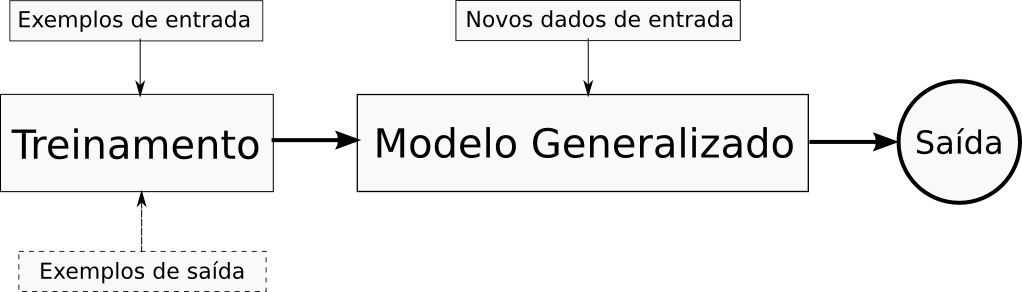
\includegraphics[scale=0.5]{img/passoapasso}
	  \end{center}
\end{figure}


O aprendizado de máquina pode ser dividido em duas abordagens: o \textbf{aprendizado supervisionado}, onde é dado um conjunto de dados de entrada e já se sabe como a saída deve parecer, tendo a ideia de que há uma relação entre a entrada e a saída; o \textbf{aprendizado não supervisionado}, que permite abordar problemas com pouca ou até nenhuma ideia de como os resultados devem parecer, nesse caso a caixa de exemplos de saída pode não existir.

Neste trabalho, utilizaremos o aprendizado supervisionado, pois já temos um conjunto de classes gramaticais como saída esperada.

O aprendizado supervisionado permite dividir os problemas em duas categorias distintas:


\begin{itemize}
	\item \textbf{Regressão}: Tenta-se prever resultados com uma saída contínua, significando que deseja-se mapear variáveis de entrada em alguma função contínua. A \autoref{fig:demregressao} demonstra esse processo. Os círculos em vermelho são dados de exemplo, já a reta azul representa a predição feita pela regressão.
	\item \textbf{Classificação}:  Tenta-se prever resultados em uma saída discreta, ou seja, deseja-se mapear variáveis de entrada em categoriais discretas. A \autoref{fig:demclassificacao} demonstra esse processo. Tem duas classes diferentes, as representadas pelos círculos amarelos e pelas cruzes vermelhas, já o contorno em verde representa o resultado da classificação sobre esses dados de exemplo.
\end{itemize}


\begin{figure}[htb]
	  \caption{Demonstração de regressão}\label{fig:demregressao}
	  \begin{center}
	      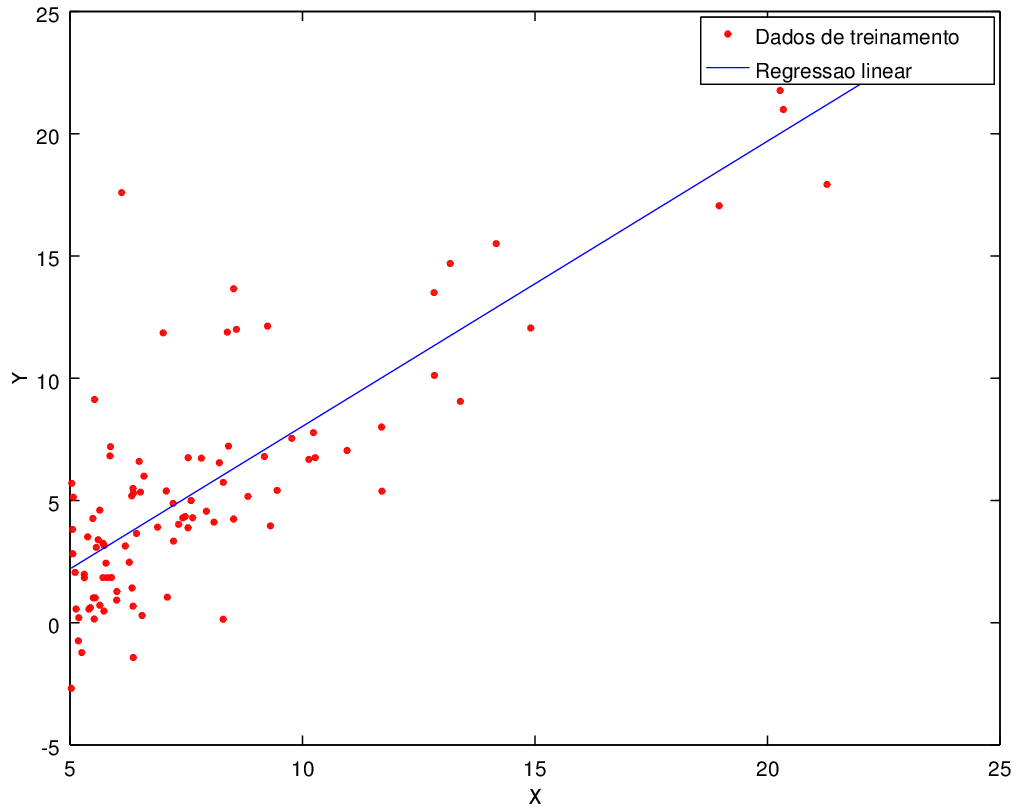
\includegraphics[scale=0.75]{img/regressao2}
	  \end{center}
	  \legend{Fonte: \citeonline{machinelearningcoursera}}
\end{figure}

\begin{figure}[htb]
  \caption{Demonstração de classificação}\label{fig:demclassificacao}
  \begin{center}
      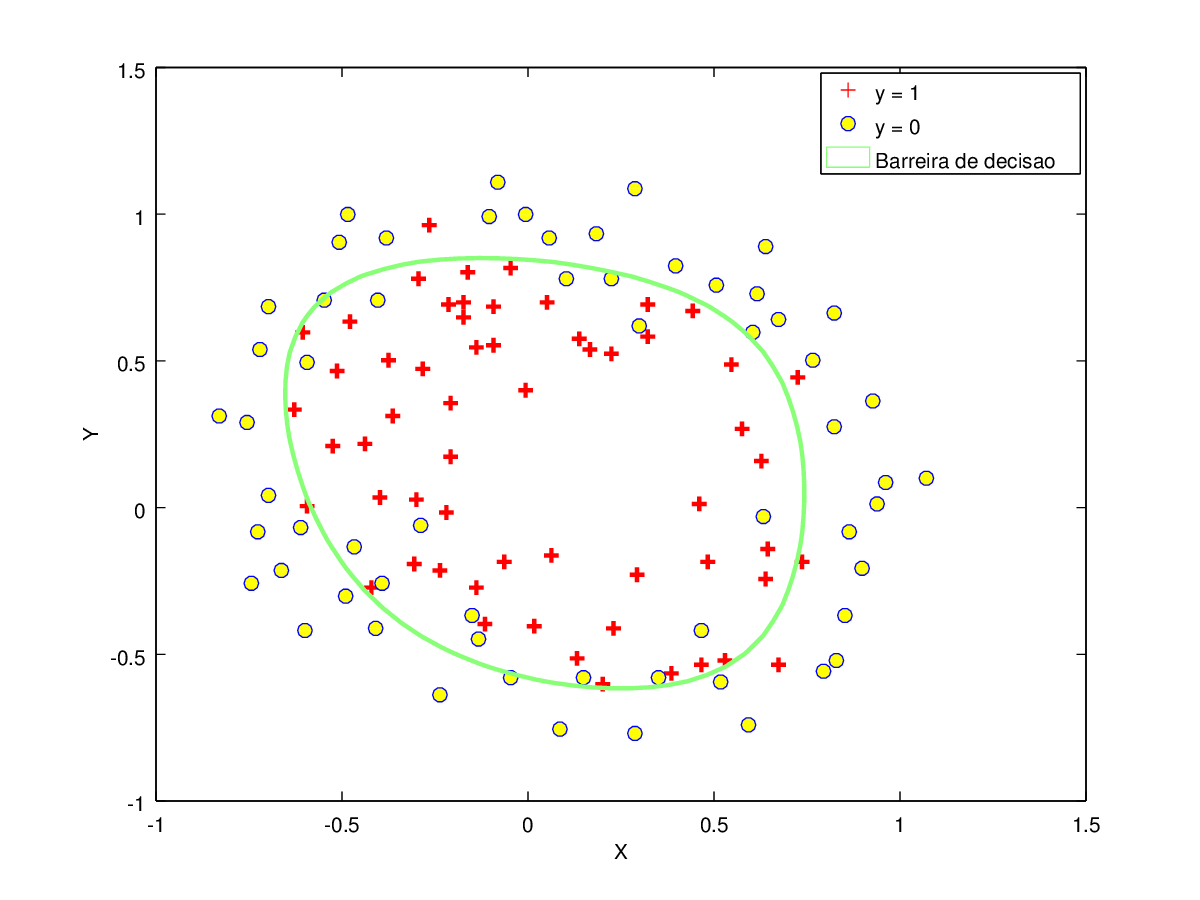
\includegraphics[scale=0.75]{img/classificacao2}
  \end{center}
  \legend{Fonte: \citeonline{machinelearningcoursera}}
\end{figure}


Logo adiante explicaremos os fundamentos de classificação e uma técnica para resolver esse problema chamada de regressão logística \cite{hosmer2004applied}. E em virtude de apresentar conceitos fundamentais a serem aplicados posteriormente nas redes neurais profundas, falaremos um pouco mais sobre regressão logística, e também sobre propriedades importantes que serão referenciadas durante todo o trabalho.

\subsection{Classificação}

Em um problema de classificação, nossa saída \textit{Y} vai ser um vetor com valores sendo apenas zero ou um.

\begin{equation}
Y \in \{0, 1\} \nonumber
\end{equation}

A equação acima está tratando apenas duas classes. Sendo assim, esse problema é chamado de classificação binária. Para resolver esse problema, um método que pode ser utilizado é regressão logística.

A fim de simplificar o uso das variáveis, faremos o uso de uma notação que é normalmente utilizada em textos de aprendizado de máquina, ela pode ser vista na \autoref{tab:classificacaonomenclatura}.

\begin{table}[!htb]
\caption{Notação utilizada para classificação} \label{tab:classificacaonomenclatura}
\begin{center}
\begin{tabular}{ll}
  \toprule
  $X$ & dados de entrada ou \textit{features} \\
  $Y$ & dados de saída \\
  $X_j^{(i)}$ & o valor da \textit{feature} \textit{j} no i-ésimo exemplo de treinamento \\
  $X^{(i)}$ & o vetor coluna de todas as \textit{features} no i-ésimo exemplo de treinamento \\
  $m$ & número de exemplos de treinamento \\
  $n$ & $|X^{(i)}|$, o número de \textit{features} \\
  $(x, y)$ & um exemplo de treinamento \\
  $(X^{(i)}, Y^{(i)})$ & o i-ésimo exemplo de treinamento \\
  $\theta$ & parâmetros a serem aprendidos \\
  \bottomrule
\end{tabular}
\end{center}

\end{table}



\ \\
\ \\

\subsection{Função de hipótese}

A função de hipótese tem o objetivo de mapear funções aleatórias dentro do intervalo de saída \textit{Y}, para isso são atribuídos valores para os parâmetros $\theta$s. Essa relação está definida na \autoref{eq:funcaodehipotese}. Observe que ela tem apenas dois parâmetros. Na realidade uma hipótese pode ter vários parâmetros relacionados com os dados de entrada \textit{X}, se tiver \textit{n} dados de entrada, então haverá \textit{n+1} parâmetros. A forma geral da função de hipótese está mostrada na \autoref{eq:funcaodehipotesegeral}.

\begin{align}
h_{\theta}(x) = &\ \theta_0 + \theta_1 x \label{eq:funcaodehipotese} \\
h_{\theta}(x) = &\ \theta_0 + \theta_1 x_1 + \theta_2 x_2 + ... + \theta_n x_n \label{eq:funcaodehipotesegeral}
\end{align}

Uma maneira de simplificar a função de hipótese é trabalhar com a definição de multiplicação de matrizes. Então a função de hipótese pode ser representada de uma forma vetorizada, como mostrado na \autoref{eq:funcaodehipotesegeralvet}. 

\begin{equation}
h_{\theta}(x) = \big[\theta_0\ \theta_1\ ...\ \theta_n\big] \times \begin{bmatrix} x_0 \\ x_1 \\ \vdots \\ x_n \end{bmatrix}  = \theta^TX \label{eq:funcaodehipotesegeralvet}
\end{equation}

Para que seja possível fazer operações de matrizes com $\theta$ e $X$, será atribuído $X_0^{(i)} = 1$ para todos os valores de $i$. Isso faz com que os vetores $\theta$ e $X^{(i)}$ combinem um com o outro elementarmente.

Portanto, nossa função de hipótese deve satisfazer a \autoref{eq:reglogicfuncaohip}.

\begin{equation}\label{eq:reglogicfuncaohip}
0 \leq h_{\theta}(x) \leq 1
\end{equation}

Para fazer com que uma entrada contínua fique nesse intervalo, é necessário utilizar uma função linear que faça esse mapeamento de modo linear, e para isso mudamos a forma da função de hipótese. A nova forma usa a função sigmoide, também conhecida como função logística.

\begin{align}
h_{\theta}(x) = & g(\theta^TX) \nonumber \\
g(z) = & \frac{1}{1 + e^{-z}} \label{eq:funcaosigmoide}
\end{align}

\begin{figure}[!htb]
  \caption{Função sigmoide}
  \label{fig:funcaosigmoide}
  \begin{center}
  \begin{tikzpicture}
  \begin{axis}[
  		width=.8\textwidth,
		scaled ticks=false,
		log ticks with fixed point,
		ymin=0,ymax=1,xmin=-10,xmax=10,domain=-10:10,
		log basis y = 10,
		xlabel=X,
      	ylabel=Y,
      	legend style={draw=none},
      	samples=200,
    ]
    \addplot[blue] { 1 / (1 + pow(e, -x))};
  \end{axis}
  \end{tikzpicture}
  \end{center}
\end{figure}

A função da \autoref{eq:funcaosigmoide} representada na \autoref{fig:funcaosigmoide} mapeia qualquer número no intervalo [0, 1], tornando isso útil para transformar qualquer valor arbitrário em uma função mais ideal para problemas de classificação.

Para calcular a função de hipótese, podemos colocar o $\theta^TX$ na função logística. Isso nos dará a probabilidade de que a saída é 1.

\begin{equation}
h_{\theta}(x) = P(y=1 | X ; \theta) = 1 - P(y=0 | X ; \theta) \nonumber
\end{equation}

Ou seja, a probabilidade de nossa predição ser 1 é o oposto da probabilidade de ser 0. Sendo assim, a soma das probabilidades para \textit{y = 0} e \textit{y = 1} deve ser 1.

Para ter uma classificação discreta podemos traduzir a saída da função de hipótese de acordo com a \autoref{eq:decisionboundary}:
\begin{align} 
h_{\theta}(x) \geq 0.5 \Rightarrow y = 1 \nonumber \\
h_{\theta}(x) < 0.5 \Rightarrow y = 0 \label{eq:decisionboundary}
\end{align}

Então, se a entrada é $\theta^TX$, isso significa que:
\begin{equation}
h_{\theta}(x) = g(\theta^TX) \geq 0.5 \quad \text{ quando } \quad \theta^TX \geq 0 \nonumber
\end{equation}

A partir disso, podemos dizer que:
\begin{align}
\theta^TX \geq 0 \Rightarrow y = 1 \nonumber \\
\theta^TX < 0 \Rightarrow y = 0 \nonumber
\end{align}

O \textbf{limite de decisão} (ou barreira de decisão) é a linha que separa a área quando \textit{y = 0} e quando \textit{y = 1}. Isso é criado pela função de hipótese. Uma observação importante é que a função de hipótese não precisa ser linear, pode ser até mesmo um círculo ou ter qualquer forma para ajustar os dados, como mostrado na \autoref{fig:demclassificacao}. Isto é, uma função de hipótese pode ter várias \textit{features}. Novas \textit{features} podem ser criadas ao combinar as \textit{features} já existentes e modificando-as. Por exemplo, se houvesse dois dados de entrada $x_1$ e $x_2$, seria possível criar a função de hipótese:

\begin{equation}
\nonumber
h_{\theta}(x) = \theta_0 + \theta_1 x_1 + \theta_2 x_2 + \theta_3 x_1 x_2 + \theta_4 x_1^2 + \theta_5 x_2^2 + \theta_6 x_1^2 x_2^2 + \cdots
\end{equation}

Todavia, essa abordagem pode gerar problemas de desempenho. Algumas \textit{features} podem também acabar se tornando obsoletas e não ajudar em nada no resultado final, tornando seu cálculo inútil. Mas o principal problema dessa abordagem é o \textit{overfitting}, que faz com que a função de hipótese não generalize sobre dados desconhecidos. Esse problema será tratado na \autoref{subsec:regularizacao}.


\subsection{Função de custo}

Para medir a precisão da função de hipótese é necessário uma função que diga o quão precisa aquela hipótese é. Tal função é denominada de função de custo. Com ela, é feita uma média de todos os resultados das hipóteses com a entrada \textit{X} comparada com o valor objetivo \textit{Y}. Ela pode ser expressa como na \autoref{eq:funcaodecusto}.

\begin{equation}
\label{eq:funcaodecusto}
J(\theta) = \frac{1}{m}\sum\limits_{i=1}^{m}Custo(h_{\theta}(x^{(i)}, y^{(i)}))
\end{equation}

Onde,


\begin{align}
 Custo(h_{\theta}(x^{(i)}, y^{(i)})) = \left\{
  \begin{array}{l l} 
    -log(h_{\theta}(x)) & \quad \text{se } y=1 \\
    -log(1 - h_{\theta}(x)) & \quad \text{se } y=0 \label{eq:funcaocusto}
  \end{array} \right.
\end{align}


A \autoref{eq:funcaocusto} captura a intuição de que se $h_\theta(x) = 0$, mas $y = 1$, então o algoritmo de aprendizado será penalizado por um custo muito alto. A \autoref{fig:logfunctions} demonstra os dois respectivos casos dessa equação.


\begin{figure}[!htb]
  \caption{Representação dos casos da função de custo}
  \label{fig:logfunctions}
  \begin{center}
  \begin{tikzpicture}

  % \draw[step=1cm,gray,very thin] (0,0) grid (11.3, 9.5);

  \begin{axis}[
  		width=.8\textwidth,
		scaled ticks=false,
		xlabel=$x$,
		log ticks with fixed point,
		ymin=0,ymax=2,xmin=0,xmax=1,domain=0:1,
		log basis y = 10,
        ylabel=$custo$,
      	legend style={draw=none},
      	samples=200,
    ]
    \addplot[blue] { - ln(x)/ln(10)};
    \addplot[orange] { - ln(1 - x)/ln(10)};
    \addlegendentry{y = 1}
    \addlegendentry{y = 0}
  \end{axis}
  \end{tikzpicture}
  \end{center}
\end{figure}


O quanto mais a função de hipótese está longe de \textit{y}, maior é a saída da função de custo. Se a função de hipótese é igual a \textit{y}, então o custo é 0.

Podemos simplificar a \autoref{eq:funcaocusto} com dois casos condicionais em apenas um caso:

\begin{equation} 
\label{eq:funcaodecustosimplificada}
Custo(h_{\theta}(x), y) = -ylog(h_{\theta}(x)) - (1-y)log(1 - h_{\theta}(x))
\end{equation}

Nota-se que quando \textit{y} é igual a 1, o segundo termo será 0 e não afetará o resultado. E quando \textit{y} é igual a 0, o primeiro termo será 0 e não afetará o resultado. Aplicando a \autoref{eq:funcaodecustosimplificada} na função de custo da equação \autoref{eq:funcaodecusto}, podemos reescrevê-la como a equação \autoref{eq:funcaodecustofinal} ou na versão vetorizada da \autoref{eq:funcaodecustovet}.

\begin{equation}
\label{eq:funcaodecustofinal}
J(\theta) = - \frac{1}{m}\sum\limits_{i=1}^{m}\Big( y^{(i)}log(h_{\theta}(x^{(i)})) + (1-y^{(i)})log(1 - h_{\theta}(x^{(i)})) \Big)
\end{equation}

\begin{equation}
J(\theta) = - \frac{1}{m}\Big( log(g(X\theta))^TY + log(1 - g(X\theta))^T(1 - Y) \Big) \label{eq:funcaodecustovet}
\end{equation}

O objetivo da regressão logística é minimizar a função de custo em relação aos parâmetros $\theta$s. Usando dois parâmetros é possível visualizar uma função de custo através do número de iterações, isso pode ser observado no exemplo da \autoref{fig:funcaodecustosurf} e da \autoref{fig:funcaodecustocontorno}. 


\begin{figure}
  \caption{Função de custo - $J(\theta_0, \theta_1)$}
  \begin{subfigure}[htb]{0.5\textwidth} 
    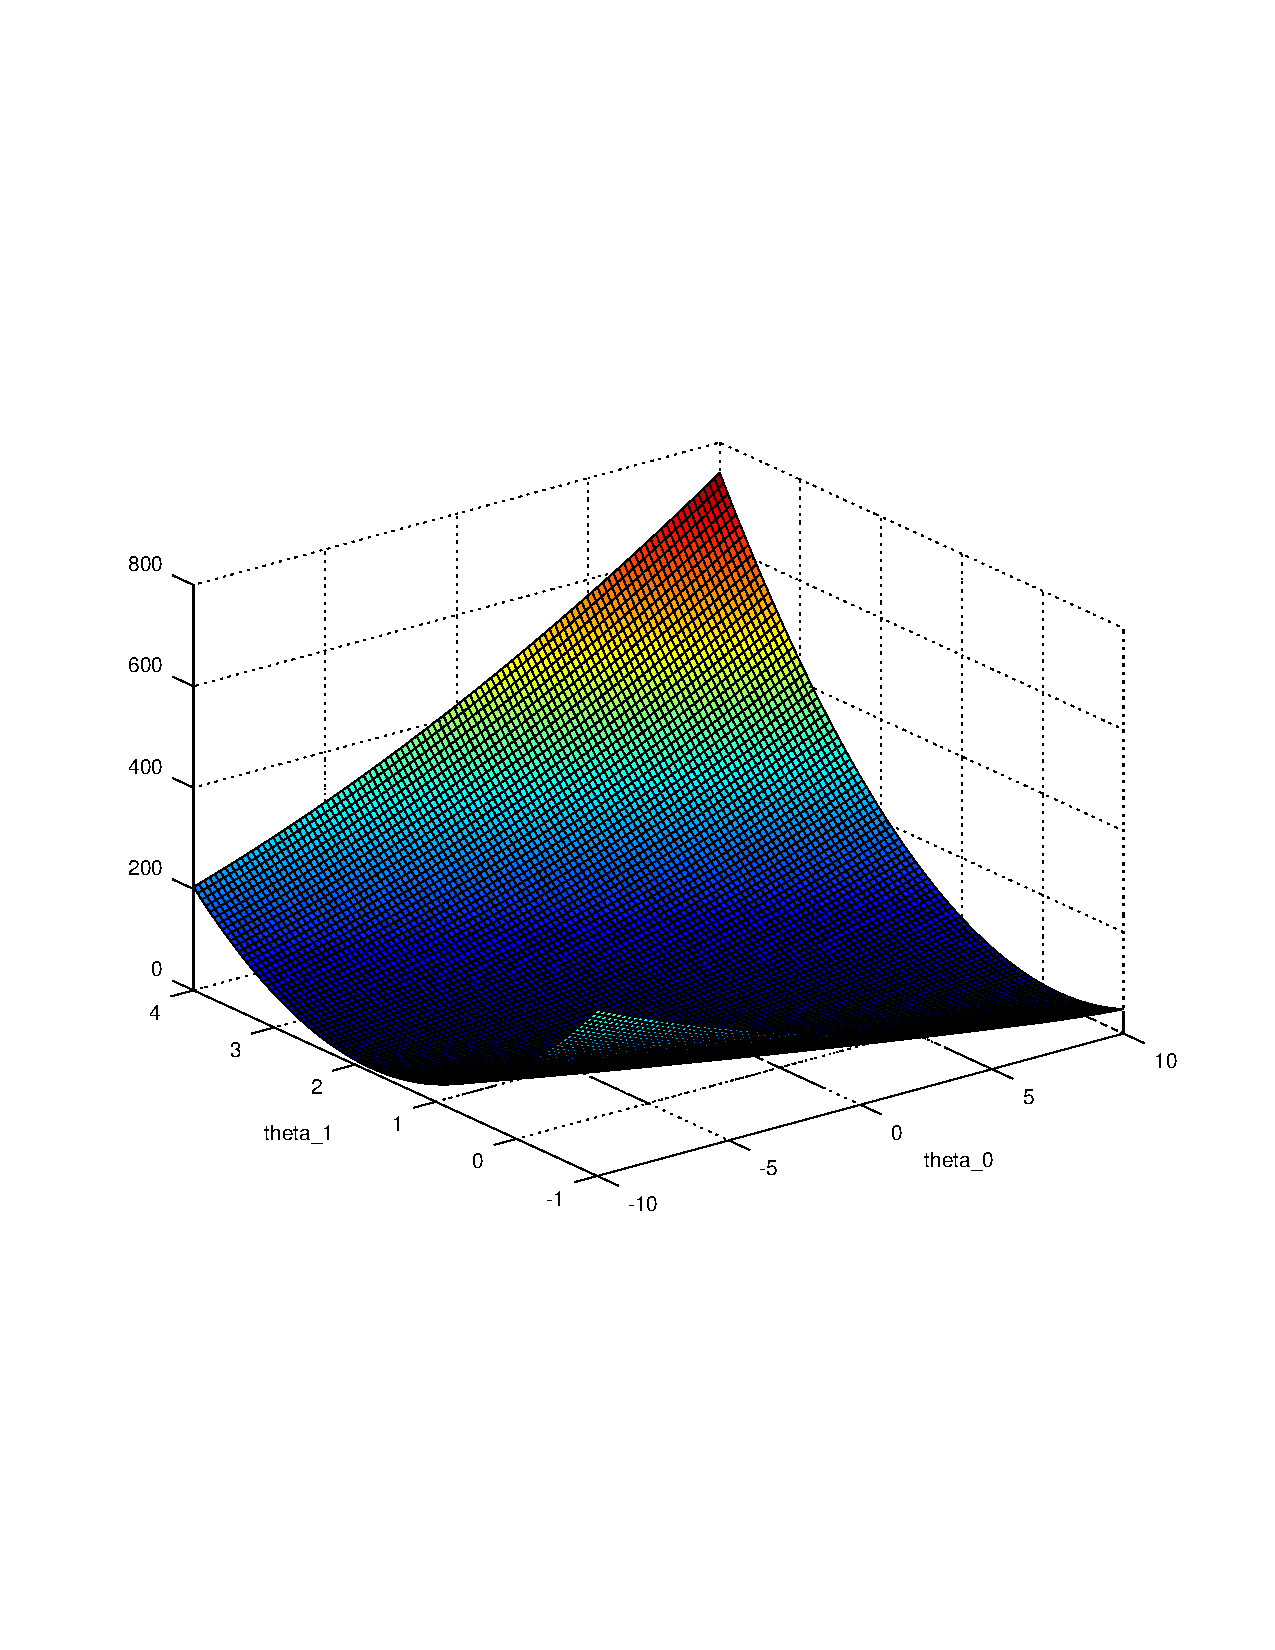
\includegraphics[width=\textwidth]{img/funcaodecustosurf} 
    \caption{Gráfico de superfície} \label{fig:funcaodecustosurf}
  \end{subfigure} 
  %
  \begin{subfigure}[htb]{0.5\textwidth}
    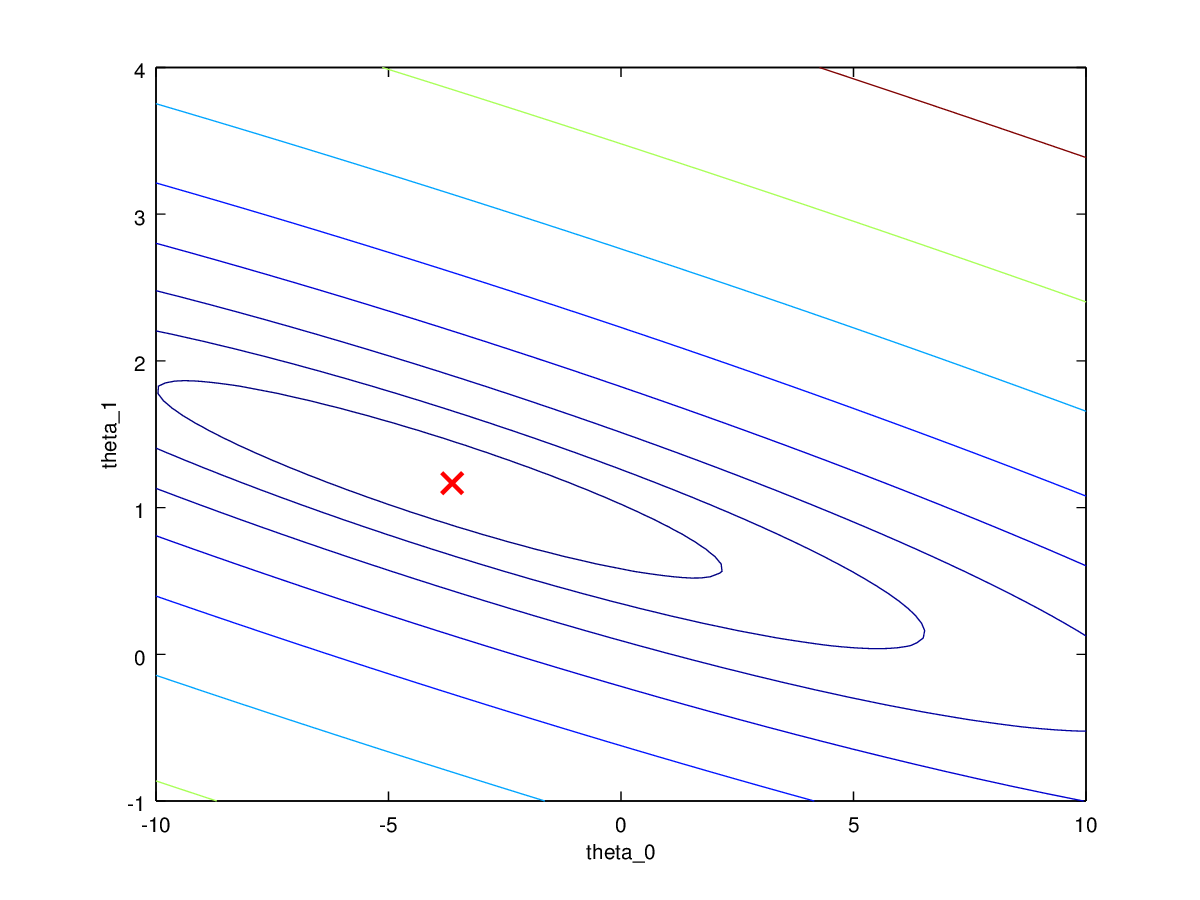
\includegraphics[width=\textwidth]{img/funcaodecustocontorno} 
    \caption{Gráfico de contorno} \label{fig:funcaodecustocontorno}
  \end{subfigure} 

  \legend{Fonte: \citeonline{machinelearningcoursera}}
\end{figure}


\subsection{Minimização da função de custo}

Para essa tarefa é necessário a aplicação de um algoritmo que pega a função de custo e tente minimizá-la, e por fim retorne os valores dos parâmetros $ \theta $s aprendidos. Com isso, estaremos melhorando nossa função de hipótese. 

Um dos algoritmos mais utilizados para essa tarefa é o \textbf{Gradiente Descendente} \cite{michalski2013machine}. Seu funcionamento baseia-se em seguir a derivada da função de custo em relação aos parâmetros $\theta$s alternadamente, com isso a encosta da tangente dará a direção para seguir adiante. Além disso, é aplicada uma taxa de aprendizagem $ \alpha $ a cada iteração, para tentar controlar a convergência.

Seu funcionamento é descrito pelo algoritmo \ref{eq:gradientedesc}.

repita até convergir \{
\begin{equation}
\label{eq:gradientedesc}
\quad \theta_j := \theta_j - \alpha \frac{\partial}{\partial\theta_j} J(\theta)
\end{equation}
\quad\quad\quad \}

Ao trabalhar sobre a derivada parcial da função de custo, podemos chegar na \autoref{eq:gradientefinal} e adiante na versão vetorizada na \autoref{eq:gradientefinalvet}. 

\begin{equation}
\quad \theta_j := \theta_j - \alpha \sum\limits_{i=1}^{m}\Big(h_{\theta}(x^{(i)}) - y^{(i)} \Big) x_j^{(i)} \label{eq:gradientefinal}
\end{equation}

\begin{equation}
\quad \theta := \theta - \frac{\alpha}{m}X^T(g(X\theta) - Y) \label{eq:gradientefinalvet}
\end{equation}

Na \autoref{fig:funcgraddesc} é possível visualizar esse funcionamento sobre os parâmetros. Observe que nesse caso o algoritmo consegue convergir para o mínimo global, porém em alguns casos (dependendo de nossa taxa de aprendizagem $ \alpha $) pode-se convergir para um mínimo local como mostrado na \autoref{fig:funcgraddescnot}. Basicamente, se $\alpha$ for um valor muito alto, os passos para o mínimal ótimo serão grandes e portanto o risco de divergência será maior, caso seja muito baixo, os passos para o mínimal ótimo serão pequenos e portanto irá demorar muito para convergir. \citeonline{machinelearningcoursera} diz para testar manualmente a taxa de aprendizagem, começando com 0,001 e ir multiplicando por 10 esse valor até atingir uma divergência no resultado. Sendo assim, é possível analisar o melhor valor da taxa de aprendizagem e selecioná-la para o treinamento definitivo. Além disso, para o Gradiente Descendente convergir, é necessário que a função de custo seja convexa.

\begin{figure}
  \caption{Funcionamento do Gradiente Descendente}
  \begin{subfigure}[htb]{0.5\textwidth} 
    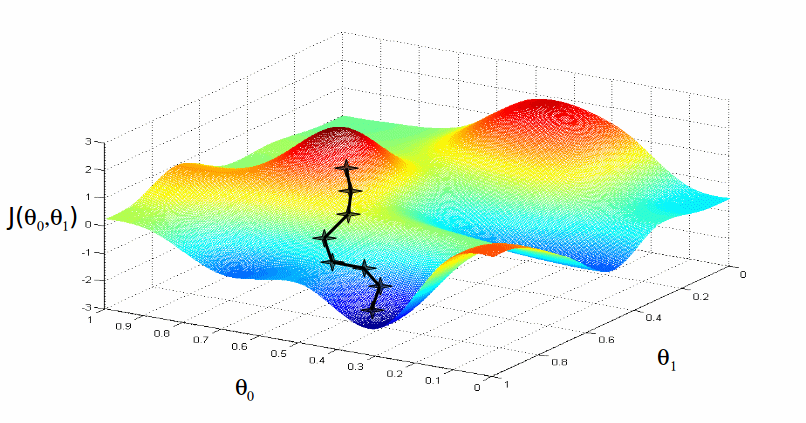
\includegraphics[width=\textwidth]{img/funcgraddesc1}
    \caption{Convergindo para uma mínimo global} \label{fig:funcgraddesc}
  \end{subfigure}
  %
  \begin{subfigure}[htb]{0.5\textwidth} 
    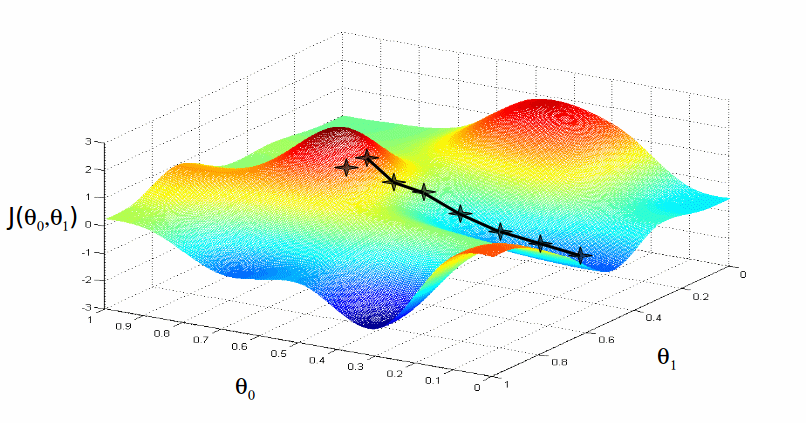
\includegraphics[width=\textwidth]{img/funcgraddesc2}
    \caption{Convergindo para uma mínimo local} \label{fig:funcgraddescnot}
  \end{subfigure}

  \legend{Fonte: \citeonline{machinelearningcoursera}}
\end{figure}

O Gradiente Descendente é apenas um dos vários algoritmos que existem para minimizar a função de custo. De acordo com \citeonline{machinelearningcoursera}, há alternativas mais sofisticadas como o Gradiente Conjugado, Broyden–Fletcher–Goldfarb–Shanno (BFGS) e Limited-memory-BFGS (L-BFGS), onde além de serem mais rápidos que o Gradiente Descendente, não é preciso selecionar manualmente o valor de $\alpha$. Mas, também é sugerido que não devemos tentar codificar esses algoritmos, visto que são mais complexos e requerem um bom conhecimento de cálculo numérico, onde ao invés podemos usar bibliotecas otimizadas que implementam esses algoritmos.


\subsection{Classificação multiclasse}

O \ac{pos} Tagging é um problema de classificação multiclasse, onde deve-se etiquetar uma palavra em uma de várias categorias gramaticais possíveis. É possível fazer isso ao expandir nossa definição para que a saída seja $Y = \{0, 1, ..., n\}$. Nesse caso, é dividido o problema em \textit{n + 1} problemas de classificação binária e em cada um será feito a predição da probabilidade de que $y$ é membro de uma dessas classes.
\begin{align}
h_{\theta}^{(0)}(X) =&  P(y=0 | X ; \theta) \nonumber \\
h_{\theta}^{(1)}(X) =&  P(y=1 | X ; \theta) \nonumber \\
\vdots & \nonumber \\
h_{\theta}^{(n)}(X) =&  P(y=n | X ; \theta) \nonumber
\end{align}

E então escolhe-se a classe com o valor de hipótese mais alto: $ \max_i(h_{\theta}^{(i)}(X)) $.


\subsection{Regularização}\label{subsec:regularizacao}

Regularização é uma técnica importante para resolver o problema de \textit{overfitting}.

Quando se trabalha com abordagens de aprendizagem supervisionada, tem-se dois problemas que podem ocorrer dependendo das \textit{features} escolhidas. O \textbf{\textit{underfitting}} ocorre quando a forma da função de hipótese mapeia mal a tendência dos dados. Isso é causado por uma função que é muito simples ou que usa poucas \textit{features}. Em contrapartida, \textbf{\textit{overfitting}} é causado por uma função de hipótese que encaixa os dados avaliados mas não generaliza bem para classificar novos dados. É usualmente causado por uma função complexa que cria muitas curvas e ângulos desnecessários.

\begin{figure}
  
  \caption{Exemplo de \textit{underfitting} e \textit{overfitting}} \label{fig:exemplounderover}
  
  \begin{subfigure}[htb]{0.5\textwidth}
    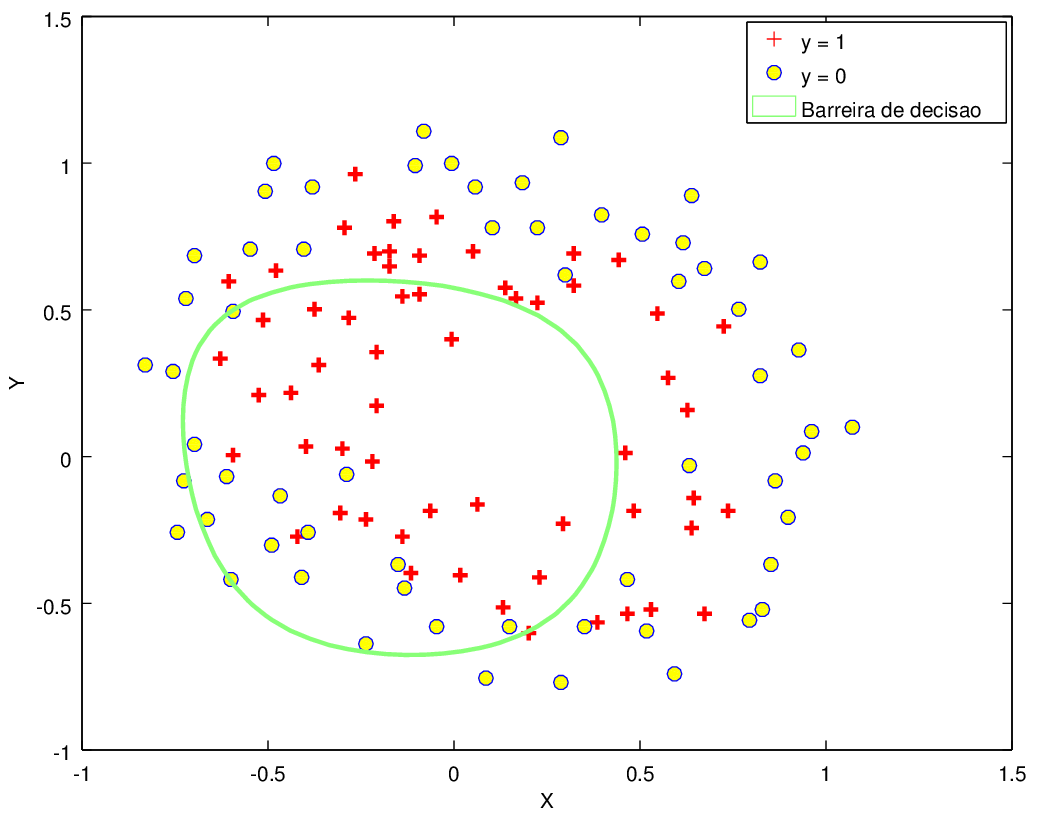
\includegraphics[width=\textwidth]{img/underfittingex}
    \legend{(a) \textit{underfitting}} 
  \end{subfigure}
  %
  \begin{subfigure}[htb]{0.5\textwidth}
    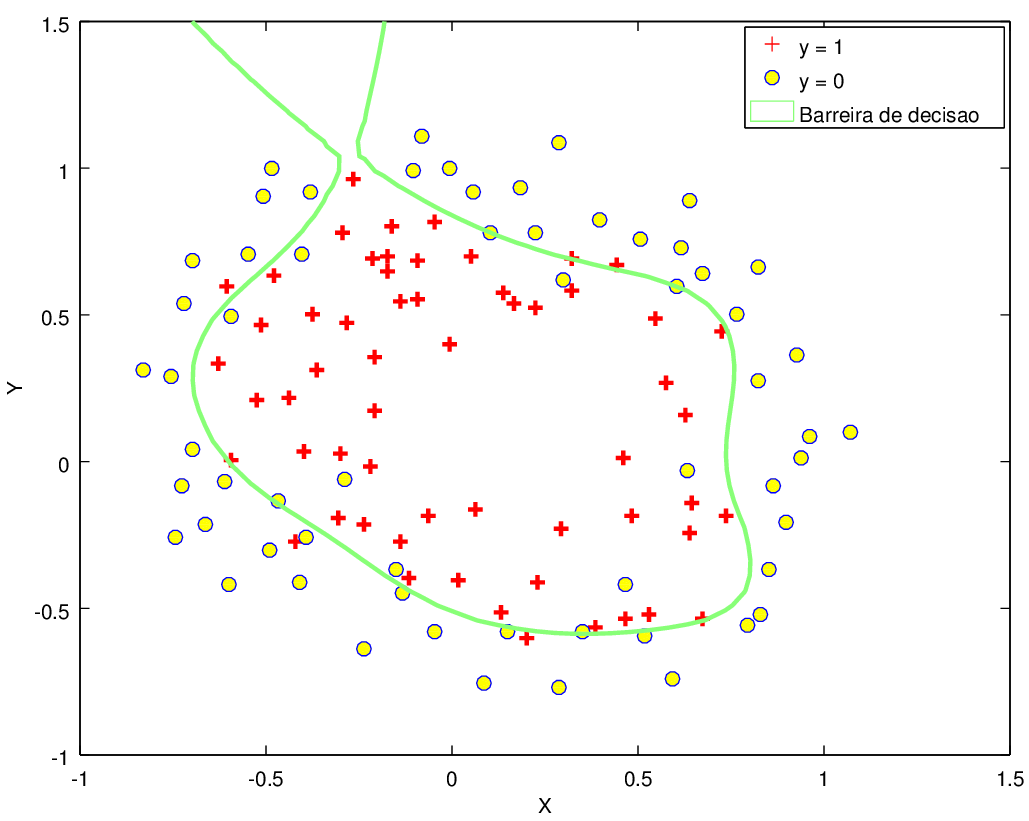
\includegraphics[width=\textwidth]{img/overfittingex}
    \legend{(b) \textit{overfitting}}
  \end{subfigure}

  \legend{Fonte: \citeonline{machinelearningcoursera}}
\end{figure}

Uma boa classificação para o conjunto de dados mostrados na \autoref{fig:exemplounderover} é o exemplo mostrado na \autoref{fig:demclassificacao}.

Segundo \cite{machinelearningcoursera}, há duas opções principais para resolver o problema de \textit{overfitting}:

\begin{alineas}
	\item Reduzir o número de \textit{features}:
		\begin{alineas}
			\item Manualmente selecionar quais \textit{features} usar;
			\item Usar um algoritmo de seleção de modelo.
		\end{alineas}
	\item Aplicar regularização:
		\begin{alineas}
			\item Manter todos as \textit{features}, mas reduzir os parâmetros $\theta_j$.
		\end{alineas}
\end{alineas}

Em geral, regularização funciona bem quando há bastante features levemente úteis. Quando há \textit{overfitting} da função de hipótese, é possível reduzir a influência de alguns termos da função aumentando os seus custos. Por exemplo, caso quiséssemos eliminar a influência de $\theta_3x^3$ e $\theta_4x^4$ da \autoref{eq:funcaodehipotesereg}, poderíamos mudar a forma da função de custo. Com isso, a função de hipótese não é alterada e as \textit{features} não são eliminadas, como mostrado na \autoref{eq:funcaodecustoreg}.

\begin{equation} \label{eq:funcaodehipotesereg}
h_{\theta}(x) = \theta_0 + \theta_1 x^1 + \theta_2 x^2 + \theta_3 x^3 + \theta_4 x^4
\end{equation}

\begin{equation} \label{eq:funcaodecustoreg}
J(\theta) = - \frac{1}{m}\sum\limits_{i=1}^{m}\Big( y^{(i)}log(h_{\theta}(x^{(i)})) + (1-y^{(i)})log(1 - h_{\theta}(x^{(i)})) \Big)
+ \underbrace{1000 \theta_3^2 + 1000 \theta_4^2}_\text{termo de regularização}
\end{equation}

Com isso, adicionamos dois termos extras no fim da função de custo para inflar o custo de $\theta_3$ e $\theta_4$. Agora, para a função de custo chegar a zero, nós teremos que reduzir os valores de $\theta_3$ e $\theta_4$ para próximos a zero. Isso vai reduzir substancialmente o peso das \textit{features} cuja influência queremos eliminar.

É possível regularizar todos os parâmetros em um único somatório conforme mostrado na \autoref{eq:funcaodecustofinalreg}. Isso pode ser feito com a inclusão do parâmetro de regularização $\lambda$, que determina o quanto os custos dos parâmetros $\theta$s serão inflados.

\begin{equation} \label{eq:funcaodecustofinalreg}
J(\theta) = - \frac{1}{m}\sum\limits_{i=1}^{m}\Big( y^{(i)}log(h_{\theta}(x^{(i)})) + (1-y^{(i)})log(1 - h_{\theta}(x^{(i)})) \Big)
+ \frac{\lambda}{2m}\sum\limits_{j=1}^{n} \theta_j^2
\end{equation}

Observe que o índice $j$ do segundo somatório começa em $1$, isso significa que não estamos regularizando o $\theta_0$.

Como foi regularizado a função de custo, há de se regularizar o algoritmo que realiza sua minimização também. Quando é trabalhado com o Gradiente Descendente isso pode ser feito como no algoritmo \ref{eq:graddescreg}. Como na função de custo, não queremos regularizar o $\theta_0$ e então precisamos separá-lo em um outro passo.

\textit{repita até convergir \{}
\begin{align} 
\quad \theta_j := &\ \theta_j - \frac{\alpha}{m} \sum\limits_{i=1}^{m}(h_{\theta}(x^{(i)}) - y^{(i)}) x_0^{(i)} & \text{se \textit{j = 0}} \nonumber \\
\quad \theta_j := &\ \theta_j - \alpha \Big[ \frac{1}{m} \sum\limits_{i=1}^{m} (h_{\theta}(x^{(i)}) - y^{(i)}) x_0^{(i)} + \frac{\lambda}{m}\theta_j \Big] & \text{se \textit{j > 0}} \label{eq:graddescreg}
\end{align}
\textit{\quad\quad\quad \}}

Com isso a regressão logística pode ser aplicada normalmente, pois a regularização vai cuidar do \textit{overfitting}. Entretanto, para casos mais complexos, que envolve a criação de muitas \textit{features} como no caso de \ac{pos} Tagging, há uma melhor abordagem para realizar a etiquetagem. Essa abordagem é conhecida como redes neurais e ela será discutida na \autoref{sec:redesneurais}.


\section{\textit{Córpus} e seu conjunto de classes gramaticais}

\textit{Córpus} são coleções de textos agrupados. Eles são os exemplos de entrada para o treinamento dos parâmetros de um modelo. Eles podem conter informações adicionais, como classes gramaticais associadas das palavras. A anotação das palavras no córpus é feita manualmente por especialistas.

Esses conjuntos podem se diferenciar na sua granularidade, como por exemplo, podem ter diferentes classes gramaticais para nomes no plural e no singular, ou agrupar eles em uma única classe \cite{fonseca2015evaluating}. No inglês, há vários conjuntos de classes gramaticais que são amplamente utilizados, são o Penn Treebank tagset \cite{penntreebank}, CLAWS5 e CLAWS7.

Já no português, os \textit{córpus} estão evoluindo com o tempo. Embora alguns erros são encontrados neles \cite{fonseca2013mac}, eles ainda são a melhor opção devido a seu tamanho e qualidade. Os principais e mais utilizados para o treinamento supervisionado são o Mac-Morpho \cite{aluisio2003account} com cerca de um milhão de palavras, que retrata artigos publicados na Folha de São Paulo em 1994. O Tycho Brahe \cite{tychobrahe2010corpus} que também tem cerca de dois milhões de palavras de 66 textos históricos entre 1380 e 1881. Há também o Bosque \cite{afonso2002floresta}, um \textit{córpus} parseado que contém cerca de 185 mil palavras. Além desses, \cite{fonseca2015evaluating} apresenta uma versão revisada do Mac-Morpho, com classes gramaticais novas e junção de outras. Dados referentes a cada \textit{córpus} podem ser encontrados na \autoref{tab:dadoscorpus}.

\begin{table}[!htb]
\footnotesize
\centering
\caption{Dados dos \textit{córpus}}
\label{tab:dadoscorpus}
\begin{tabular}{m{4cm}m{2cm}m{2cm}m{4cm}}
  \toprule
  \textbf{Córpus} & \textbf{Sentenças}  & \textbf{Palavras}  & \textbf{Classes gramaticais}  \\
  \midrule
  Mac-Morpho original & 53,374 & 1,221,465 & 41  \\
  Mac-Morpho revisado & 49,932 & 945,958   & 26  \\
  Tycho Brahe         & 96,125 & 2.842.809 & 265 \\
  \bottomrule
\end{tabular}
\end{table}

Infelizmente esses \textit{córpus} não podem ser combinados em um só, já que eles se diferenciam no conjunto de classes gramaticais e também no seu uso associado. Uma possível alternativa para essa combinação seria o uso de uma aprendizagem não supervisionada, aplicando técnicas de clusterização.

A aprendizagem supervisionada, utilizando \textit{córpus} como entrada, tem se mostrado uma estratégia atrativa, já que pode ser usado recursos criados com boa eficiência. Devido a isso, nesse trabalho vamos utilizar três \textit{córpus}: o Mac-Morpho original; Mac-Morpho revisado e o Tycho Brahe. O conjunto de etiquetas para esses \textit{córpus} podem ser encontrados, respectivamente, em \cite{aluisio2003account}, \cite{fonseca2015evaluating} e \cite{tychobrahe2010corpus}.



\section{Representação das palavras}\label{sec:representacaodaspalavras}

Palavras\footnote{Uma palavra pode ser qualquer conjunto de caracteres, inclusive pontuações, números, etc.} podem ser representadas de várias maneiras em um modelo de aprendizagem, podendo ser até mesmo feito o uso real da palavra como uma \textit{feature}.

No entanto, uma abordagem recente que vem obtendo sucesso é a utilização de \textit{word embeddings}, elas são representação de palavras como vetores reais valorados em um espaço multidimensional \cite{turian2010word}. Elas podem ser geradas de maneiras diferentes dependendo da técnica utilizada. Abordagens clássicas baseiam-se na frequência e co-ocorrência das palavras profundas. Mas ultimamente o processo de geração tem sido feito através de redes neurais, onde é possível capturar informações sintáticas e semânticas sobre as palavras \cite{collobert2011natural}.

\textit{Word embeddings} conseguem mapear palavras em um espaço relativamente pequeno (usando algumas centenas de dimensões ou até menos) e capturam similiaridades entre as palavras (o tipo de similaridade varia com o método usado para gerá-las) de acordo com sua distância euclidiana, ou outro tipo de cálculo de similaridade entre vetores (\textit{cosine distance}, Jaccard, etc). Quando falamos que elas são similares, significa que elas tendem a serem usadas no mesmo contexto e usualmente pertencem a mesma classe gramatical, e em termos matemáticos significa que os vetores estão próximos um do outro. Além disso, palavras não vistas nos dados de treinamento não são completamente desconhecidas, pois elas tem uma representação vetorial. Por isso, espera-se que o impacto de palavras \ac{fdv} seja menor \cite{fonseca2015evaluating}.

As \textit{word embeddings} podem então ser consideradas como novas \textit{features} obtidas a partir das originais. Essa técnica tem interessado cada vez mais pesquisadores na área de \ac{pln}, e com isso novos processos de geração de \textit{word embeddings} tem surgido.

\citeonline{collobert2011natural} usa um modelo de rede neural (\ac{nlm}, do inglês) para inicializar suas representações de palavras, com isso evita-se a tarefa de \textit{engenharia de features}. Esse modelo é baseado na extração dos parâmetros aprendidos em uma rede neural treinada por \textit{Backpropagation}, onde após o treinamento, é gerada uma tabela de busca com a palavra original como chave e o vetor de \textit{features} como valor. Além disso, é mostrado a eficiência desse método em aplicações de análise sintática e semântica.

\citeonline{collobert2011natural} ainda nos mostra como extender a ideia de representação vetorial para incorporar \textit{features} discretas. Um exemplo disso é a presença de capitalização, que traz informações importantes da palavra. Esse processo pode ser feito ao criar vetores correspondentes a \textit{feature} criada. A \autoref{fig:exemplofeaturevectors} ilustra esse processo.

\begin{figure}[htb]
  \caption{Exemplo de vetores de \textit{features} de cinco dimensões representando palavras} \label{fig:exemplofeaturevectors}
  \begin{center}
      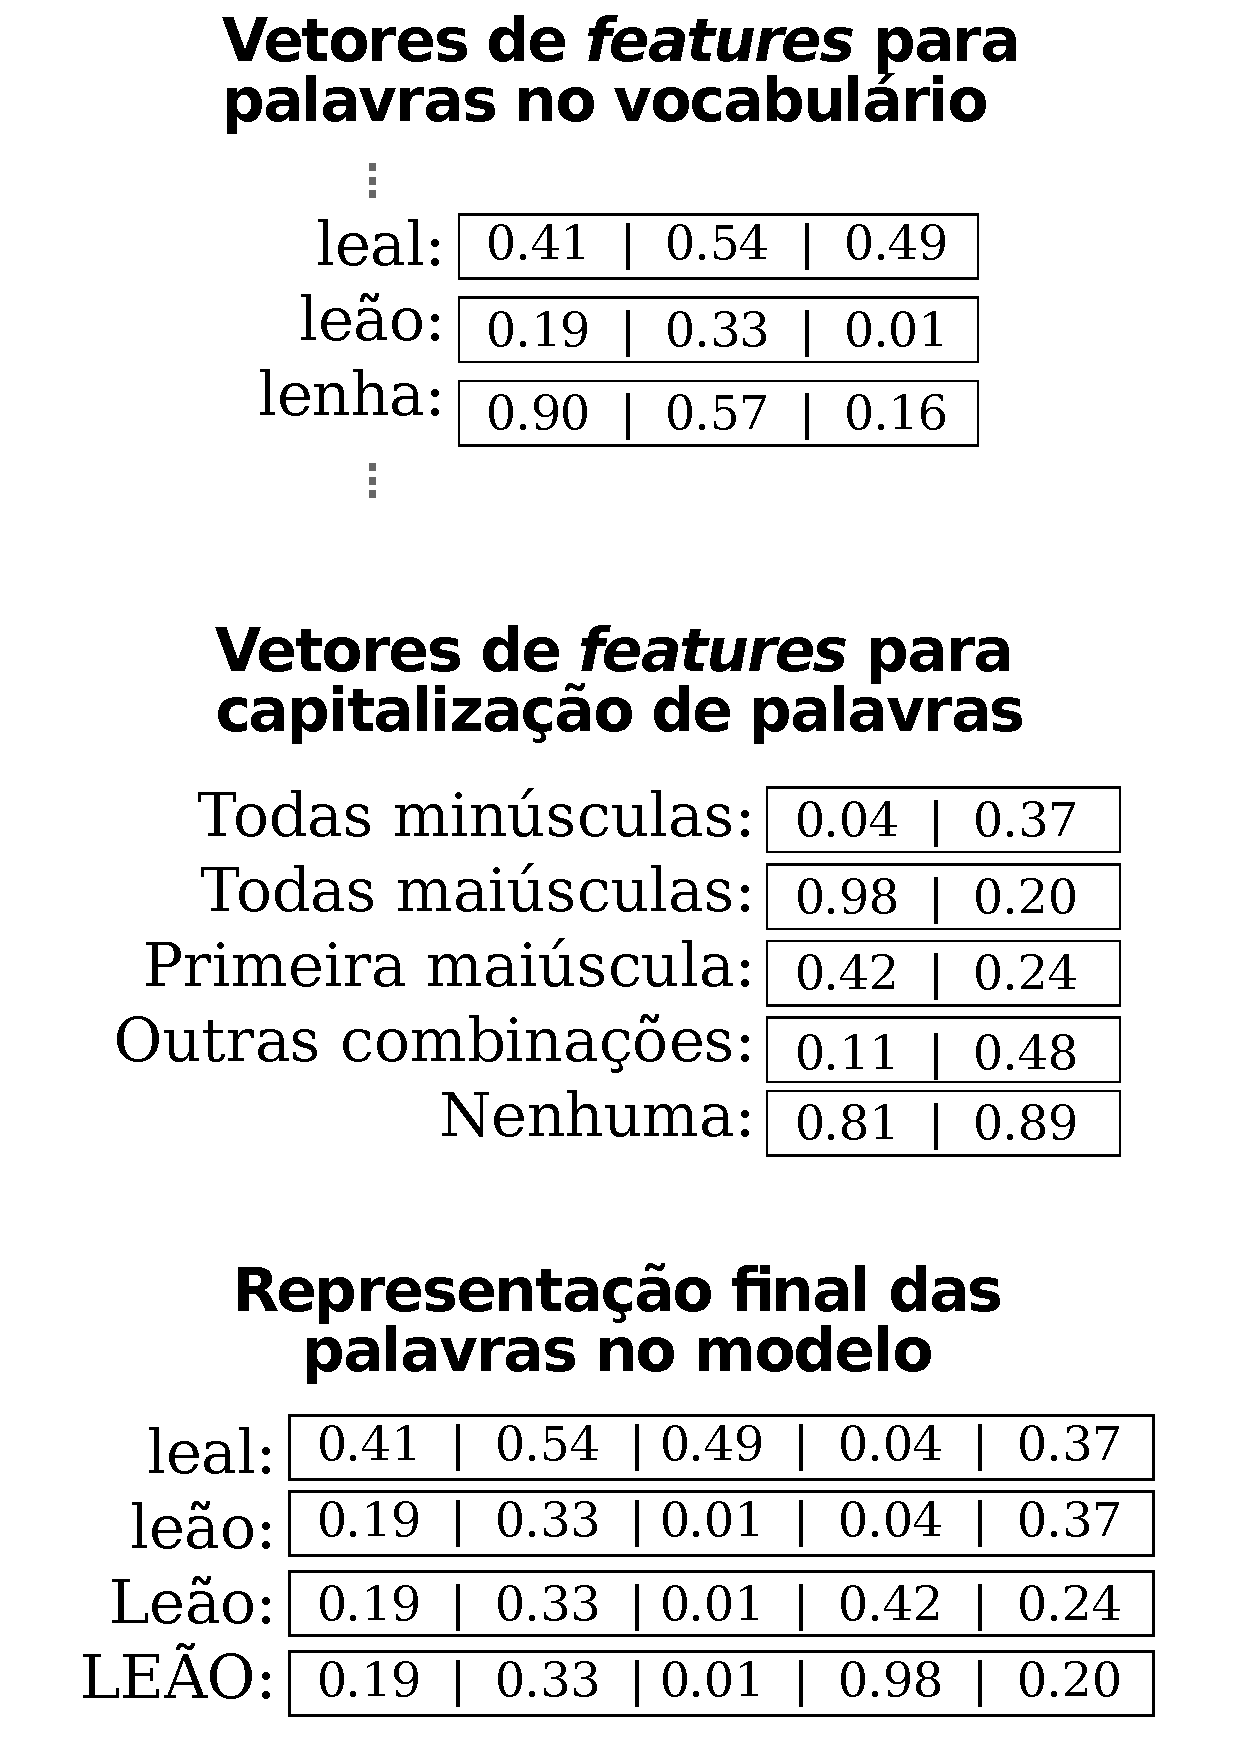
\includegraphics[scale=0.35]{img/exemplofeaturevectors.pdf}
  \end{center}
  \legend{Adapatade de: \citeonline{fonseca2015evaluating}}
\end{figure}

Outro método utilizado para a criação dos vetores é o \ac{hal} \cite{lund1996producing}. Ele é baseado na contagem de ocorrência de palavras próximas umas das outras para então obter uma grande matriz de contagem. Após finalizar a contagem, é analisada a distância euclidiana contabilizada entre as palavras do vocabulário e uma palavra alvo. Essas distâncias são então ordenadas, e os vizinhos com menores distâncias são examinados.

Além dessas, outra estratégia para gerar vetores é a modelação \ac{sg}, que tem como objetivo minimizar a complexidade computacional na geração das \textit{word embeddings}. Essa estratégia consiste em prever palavras próximas de uma dada palavra. Isso é feito usando uma palavra como entrada para o um classificador de complexidade logarítmica com uma camada de projeção contínua. A previsão é feita com um conjunto de palavras predecessoras e sucessoras, porém quanto maior for esse conjunto, maior será a complexidade computacional \cite{mikolov2013efficient}. Já que o classificador não tem uma camada oculta na sua arquitetura, ele é consideravelmente mais rápido que um modelo de rede neural. Essa estratégia é utilizada pela ferramenta \textit{word2vec}, que contém a contribuição do próprio \citeonline{mikolov2013efficient}.

A estratégia mais recente e indicada por \citeonline{deeplearningfornlp} é a utilização de \ac{glove} para representação de palavras idealizados em \cite{pennington2014glove}. Essa estratégia consiste em modelar as palavras usando representações compartilhadas entre as palavras alvo e seu contexto. Essa estratégia é atualmente o estado da arte para a representação de palavras em vetores de \textit{features}.

Portanto, para a criação de um vetor de \textit{features}, temos a transformação \textit{W} para uma palavra \textit{word}:
\begin{equation}
W:word \to \mathbb{R}^n
\end{equation}

O número de dimensões $n$ dos vetores podem variar. Em geral, quanto mais dimensões há, melhores representações podem ser alcançadas, mas se a dimensão for muito grande, o processamento pode ser demorado.

Como já mencionado, a grande vantagem em se utilizar \textit{word embeddings} é o fato dessa representação conseguir capturar informações sintáticas e semânticas das palavras. Isso pode ser visualizado através do t-SNE \cite{van2008visualizing}, uma técnica sofisticada para visualizar dados em altas dimensões.

\begin{figure}[htb]
  \caption{t-SNE: Visualização para \textit{word embeddings}}\label{fig:wordtsne}
  \begin{center}
      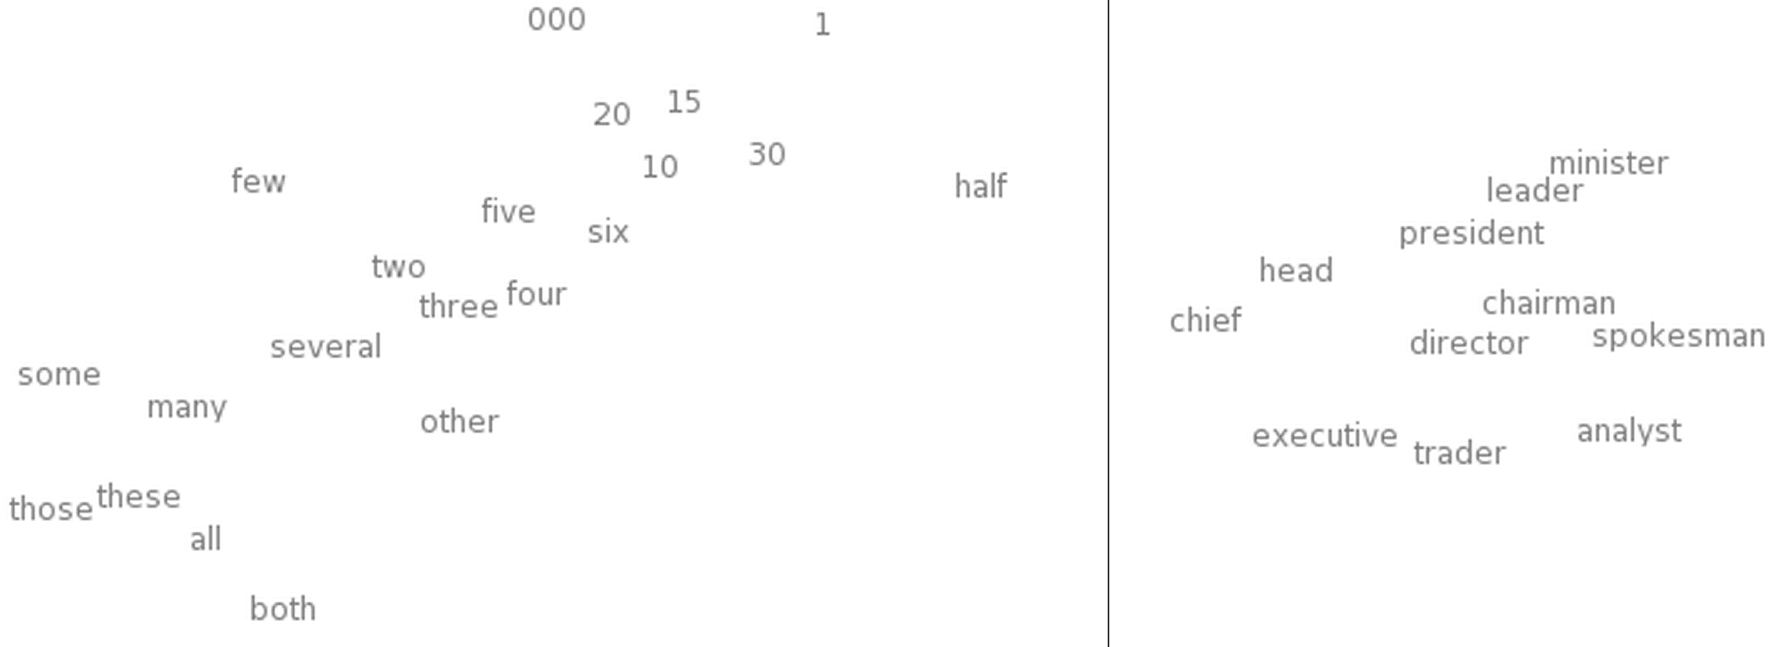
\includegraphics[scale=0.25]{img/Turian-WordTSNE}
  \end{center}
  \legend{Fonte: \citeonline{turian2010word}}
\end{figure}

Na \autoref{fig:wordtsne} podemos visualizar um tipo de mapeamento entre os sentidos intuitivos das palavras, onde na esquerda estão palavras referentes a números e na direita palavras referentes a profissões. Ou seja, palavras similares estão pertos umas das outras.

\begin{figure}[htb]
  \caption{Exemplo de palavras similares}\label{fig:palavrassimilares}
  \begin{center}
      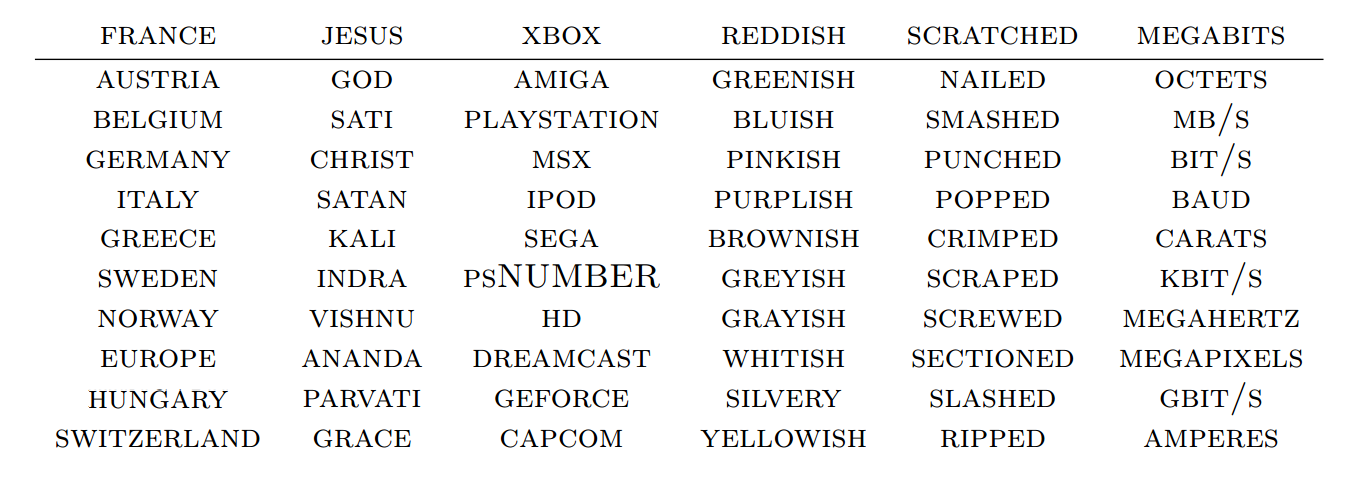
\includegraphics[scale=0.35]{img/Colbert-WordTable2}
  \end{center}
  \legend{Fonte: \citeonline{collobert2011natural}}
\end{figure}

Na \autoref{fig:palavrassimilares} temos mais alguns exemplos desse conceito, com isso podemos realizar tarefas semânticas mais facilmente. Como por exemplo: $homem + coroa = rei$, onde consegue-se realizar operações sobre os sentidos das palavras.



\section{Redes neurais}\label{sec:redesneurais}

Redes neurais tem como origem algoritmos que tentam imitar o cérebro humano. Elas eram amplamente utilizdas na década de 80 e no começo da década de 90, porém sua popularidade diminuiu no fim dessa mesma década. Ressurgiram recentemente e são o estado da arte para várias aplicações de inteligência artificial \cite{machinelearningcoursera}.

\subsection{Neurocomputação}

Há evidências de que o cérebro usa apenas um ``algoritmo de aprendizagem'' para todas diferentes funções. Cientistas já tentaram cortar (no cérebro de animais) a conexão entre as orelhas e o córtex auditivo e reconectar com o nervo óptico, o resultado foi que o córtex auditivo literalmente aprendeu a ver \cite{machinelearningcoursera}. 

Na \autoref{fig:vendocomalingua} os cientistas conseguiram fazer com que o ser humano possa enxergar através de sensores da língua conectado a uma câmera fotográfica. Já na \autoref{fig:terceiroolho}, foi implantado um terceiro olho em um sapo e após um tempo comprovou-se que o sapo definitivamente aprendeu a ver com aquele olho.


\begin{figure}
  \caption{Exemplos de representação de sensores no cérebro}
  \begin{subfigure}[htb]{0.5\textwidth} 
    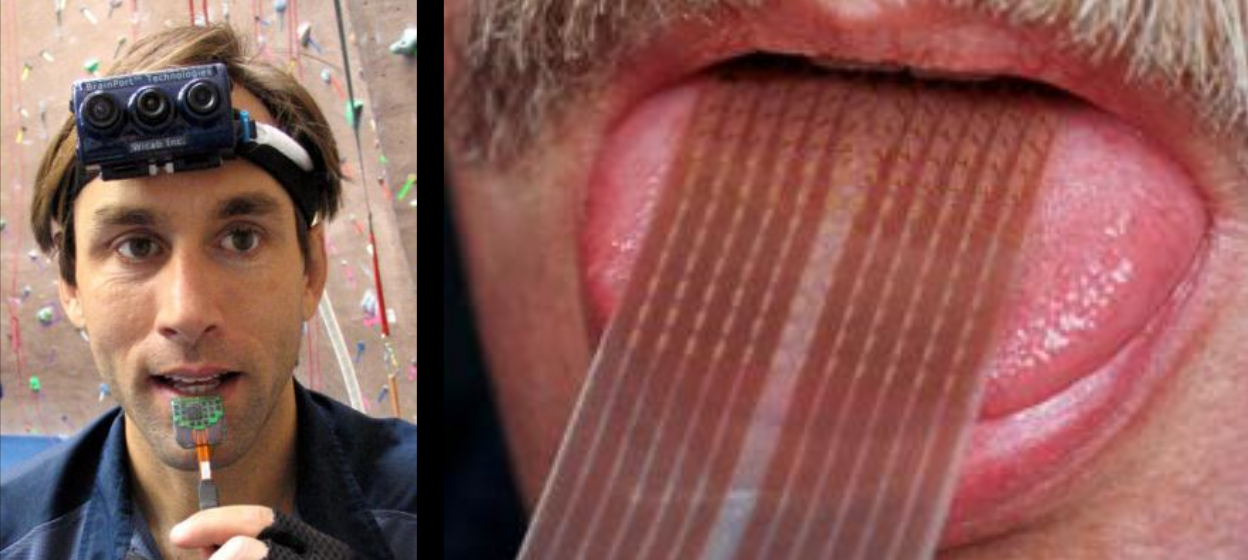
\includegraphics[width=\textwidth]{img/seeingtongue}
    \caption{Visualizando com a língua} \label{fig:vendocomalingua}
  \end{subfigure} 
  %
  \begin{subfigure}[htb]{0.41\textwidth}
    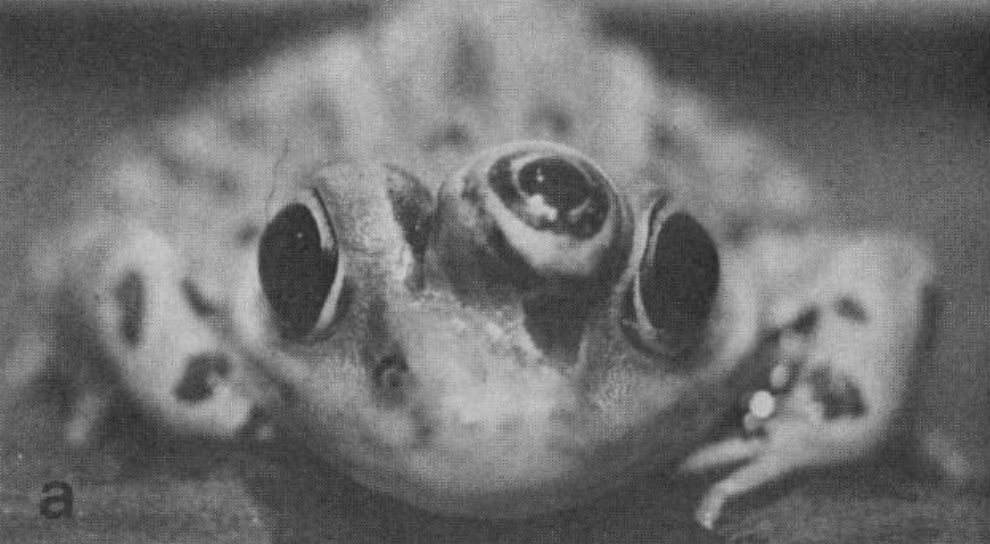
\includegraphics[width=\textwidth]{img/thirdeye}
    \caption{Implantando um terceiro olho} \label{fig:terceiroolho}
  \end{subfigure} 

  \legend{Fonte: \citeonline{ng2013unsupervised}}
\end{figure}

Esse princípio é conhecido como ``neuroplasticidade'' e tem vários exemplos e evidências de experimentos.

\subsection{Representação do modelo}

Em um nível bem simples de abstração, neurônios são basicamente unidades computacionais que recebem entradas (dendritos) como impulso elétrico que são canalizados para a saída (axônio), já o corpo celular é responsável por realizar os cálculos. Isso é ilustrado na \autoref{fig:neuronio}.

\begin{figure}
\centering
\caption{Representação de um neurônio} \label{fig:neuronio}
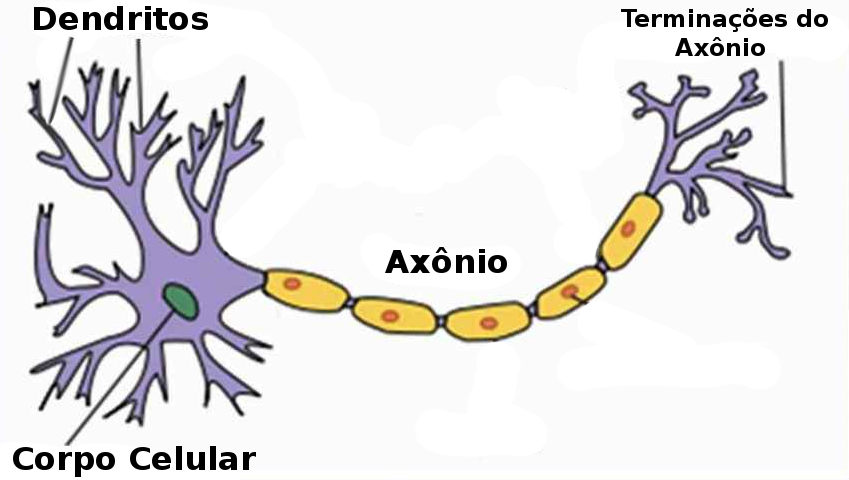
\includegraphics[width=0.75\textwidth]{img/neuron}
\legend{Fonte: \citeonline{machinelearningcoursera}}
\end{figure}


A função de hipótese pode ser representada através de um modelo de redes neurais. Nesse modelo, o $x_0$ é usualmente chamado de viés de entrada ou unidade viés (do inglês \textit{bias unit}) e ele sempre será igual a 1.

Em redes neurais, é usado a mesma função logística como em regressão logística:

\begin{equation}
\frac{1}{1 + e^{\theta^TX}} \nonumber
\end{equation}

A diferença é que em redes neurais ela é usualmente conhecida como função de ativação sigmoide. Os parâmetros $\theta$s a serem aprendidos são chamados de pesos. Visualmente, uma representação simples desse modelo se parece como a \autoref{fig:neuroniomat}. Os dados dos nodos de entrada (camada 1) vão para outro nodo (camada 2) que aplica a função de ativação, e então vão para a saída sendo a função de hipótese.

\begin{figure}
\centering
\caption{Abstração matemática de um neurônio} \label{fig:neuroniomat}
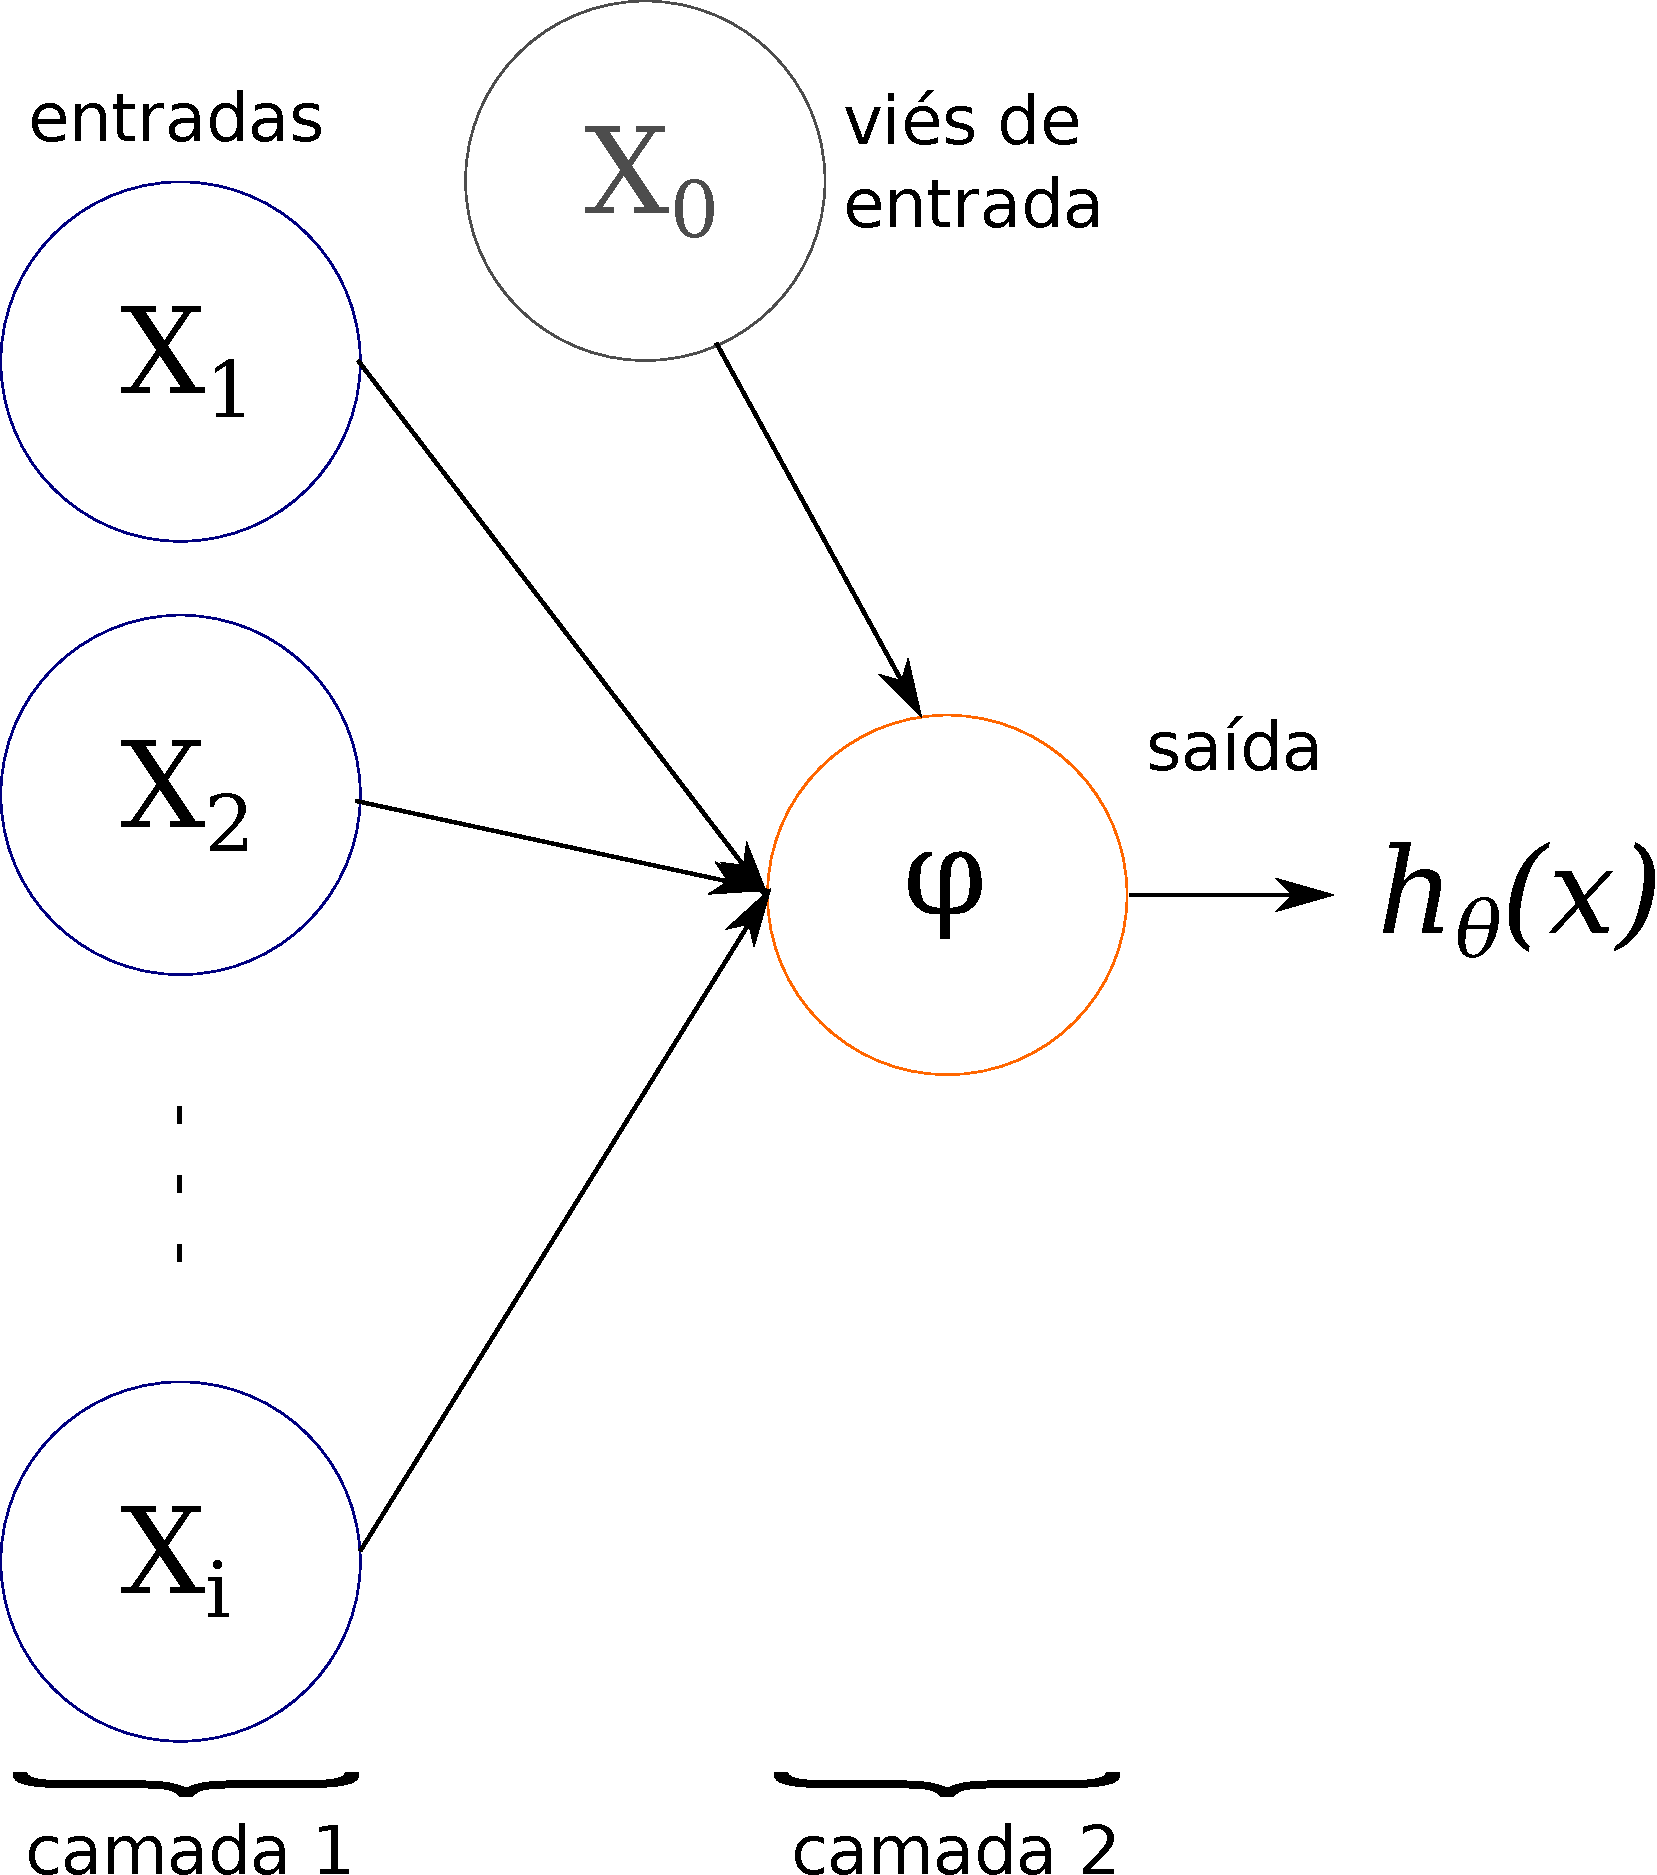
\includegraphics[width=0.75\textwidth]{img/redeneuralmat.pdf}
\end{figure}


A primeira camada é chamada de ``camada de entrada'' e a camada final de ``camada de saída'', que nos dá o valor final computado sobre a hipótese. É possível ter camadas intermediárias entre as camadas de entrada e saída chamadas de ``camadas ocultas''. 

Nomeamos os nodos das camadas intermediarias de $a_0^{(j)}, a_1^{(j)}, ..., a_n^{(j)}$ e chamamo-os de unidades de ativação. A tabela \autoref{tab:nomenclaturaredesneuras} reúne as notações geralmente usadas no contexto de redes neurais.

\begin{table}[!htb]
\caption{Notação utilizada para representação em redes neurais} \label{tab:nomenclaturaredesneuras}
\begin{center}
\begin{tabular}{m{2cm}m{12.0cm}}
  \toprule
  $\varphi$ ou $g(z)$ & função de ativação sigmoide\\
  $a_i^{(j)}$ 	   & unidade de ativação $i$ na camada $j$ \\
  $\theta^{(j)}$   & matriz de pesos mapeando funções da camada $j$ para camada $j+1$  \\
  $z_k^{(j)}$	&	parâmetros da função $g$ para a unidade de ativação $k$ na camada $j$. \\
  \bottomrule
\end{tabular}
\end{center}

\end{table}


A \autoref{fig:redeneuraloculta} mostra uma rede neural com uma camada oculta. Apesar do nodo viés não aparecer na camada oculta ele está presente nela, aliás, ele está presente e alimenta todos os nodos de todas camadas da rede (exceto a camada de saída), porém ele não recebe entradas.

\begin{figure}
\centering
\caption{Rede neural com uma camada oculta} \label{fig:redeneuraloculta}
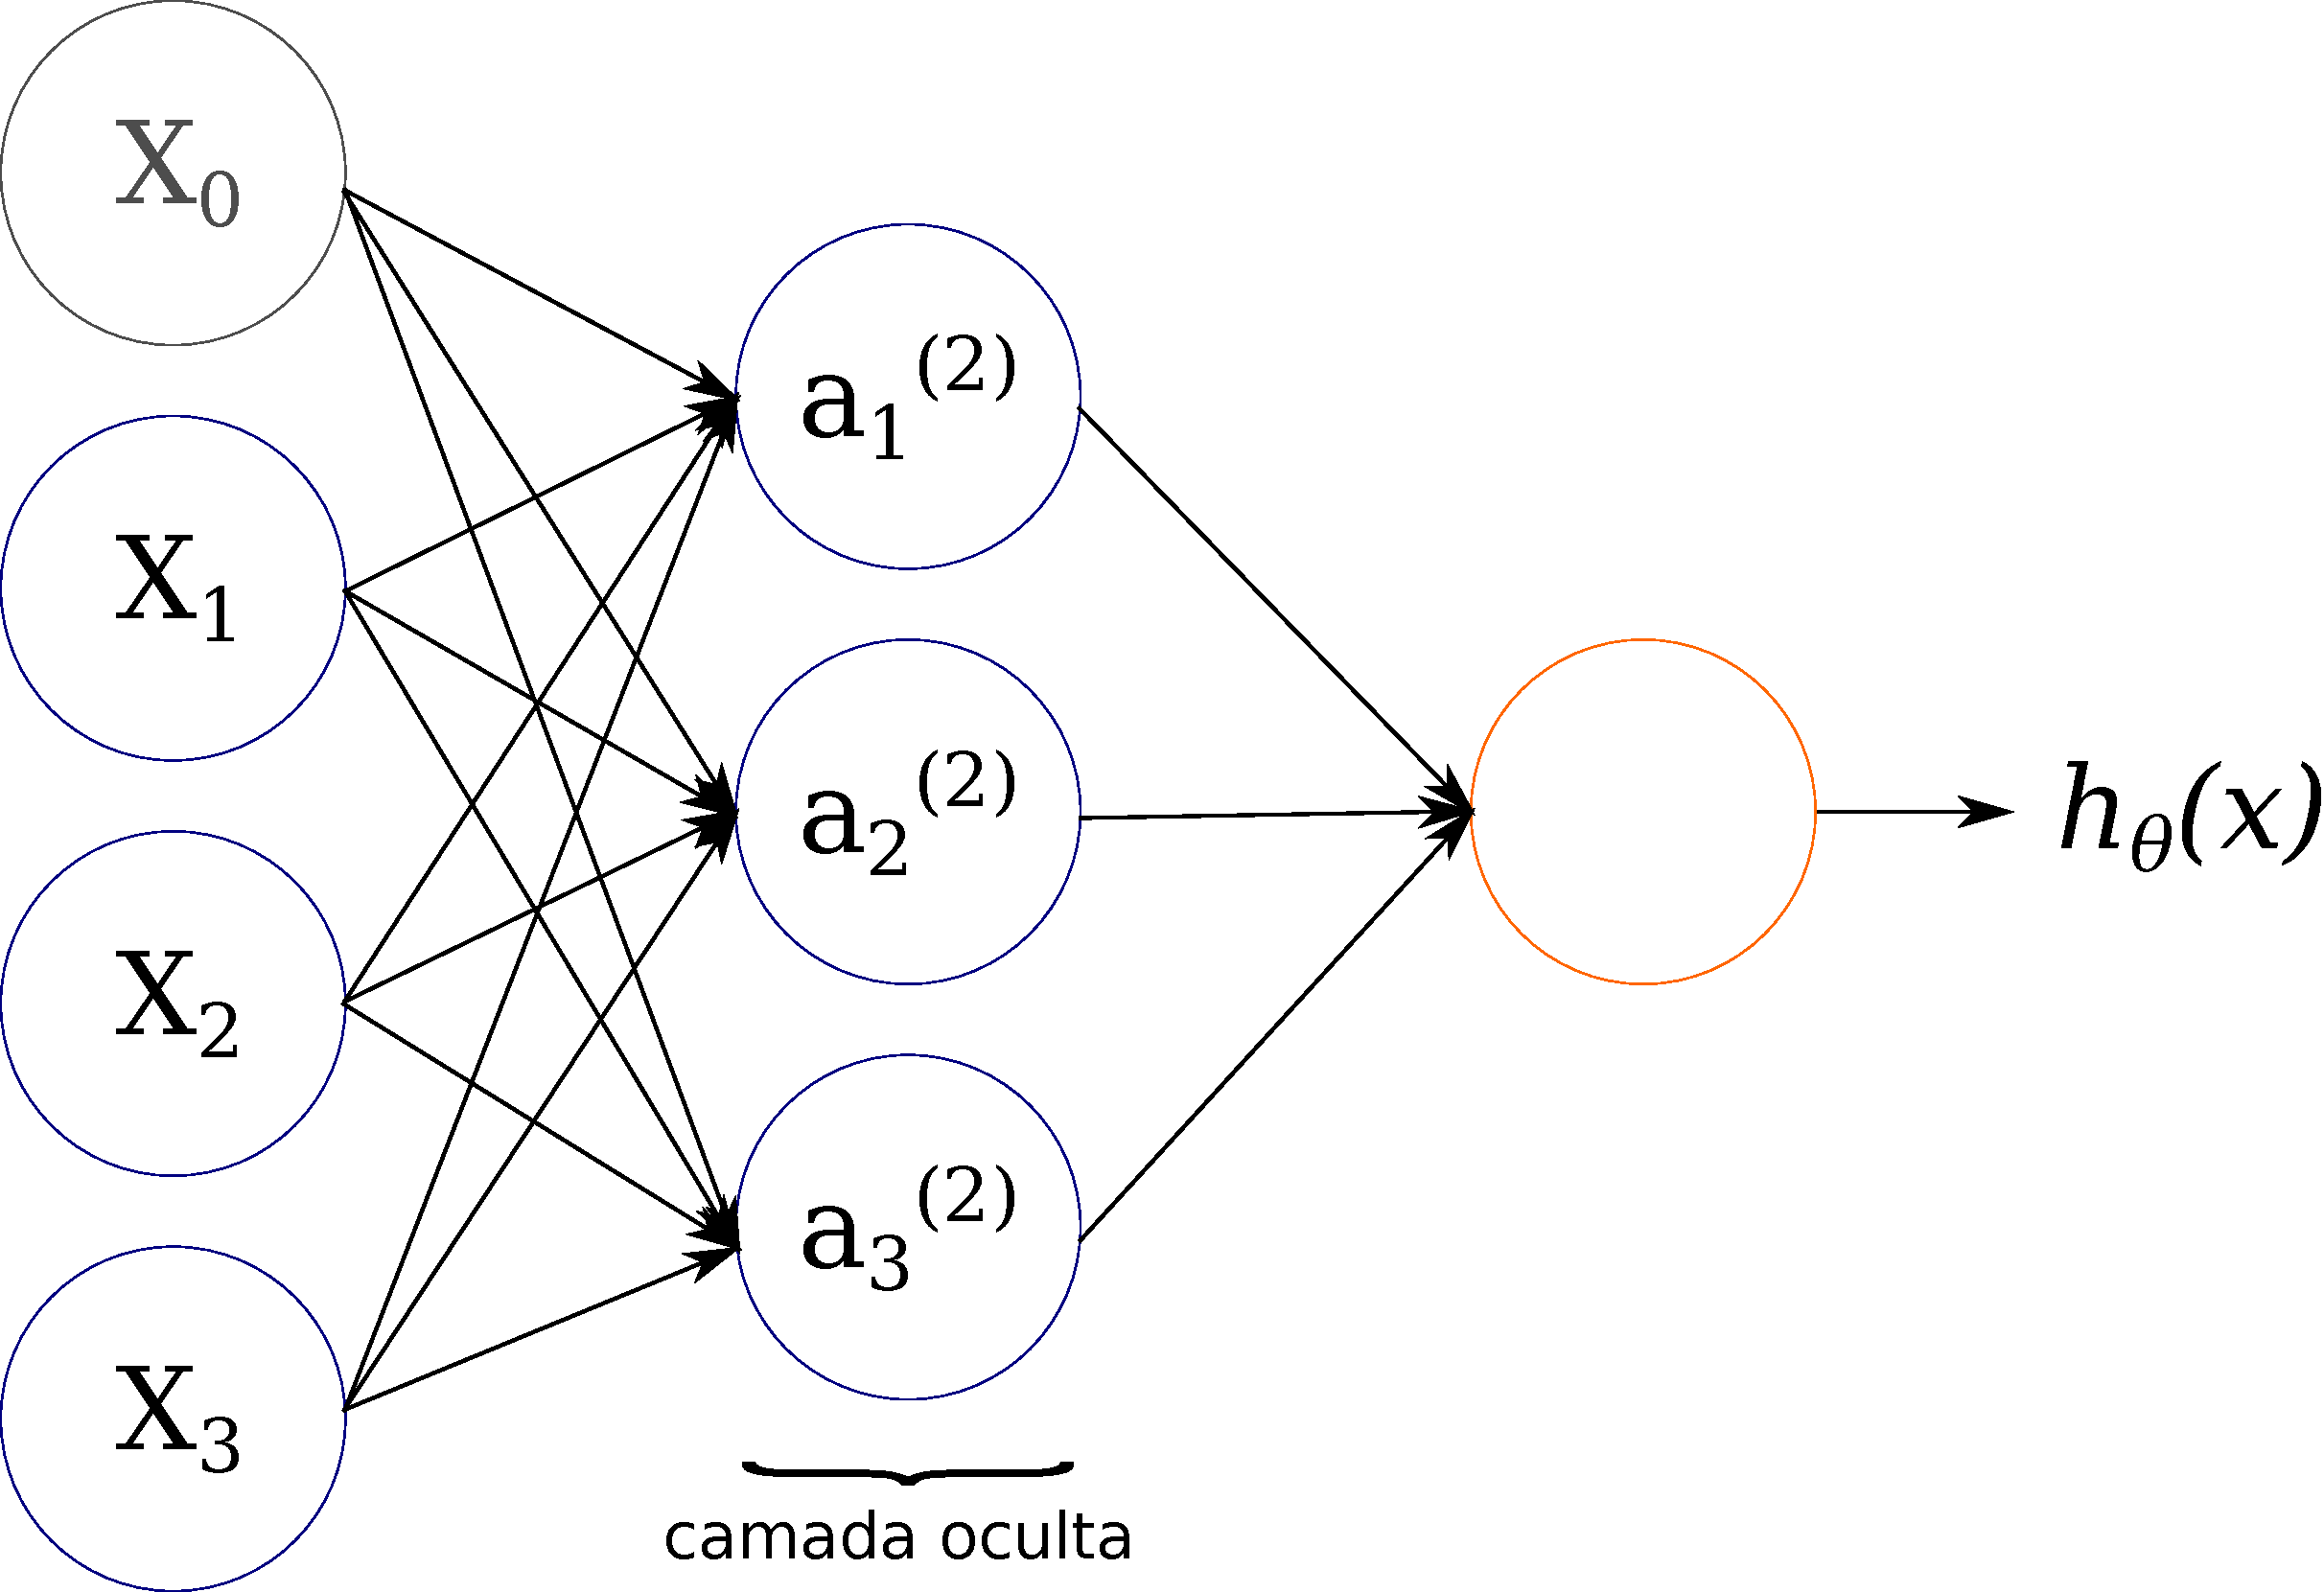
\includegraphics[width=0.75\textwidth]{img/redeneuraloculta.pdf}
\end{figure}

O valor de cada nodo de ativação pode ser obtido pelo conjunto de equações \ref{eq:conjnodosativacao}:
\begin{align}
a_1^{(2)} = g(\theta_{1,0}^{(1)}x_0 + \theta_{1,1}^{(1)}x_1 + \theta_{1,2}^{(1)}x_2 + \theta_{1,3}^{(1)}x_3) \nonumber \\
a_2^{(2)} = g(\theta_{2,0}^{(1)}x_0 + \theta_{2,1}^{(1)}x_1 + \theta_{2,2}^{(1)}x_2 + \theta_{2,3}^{(1)}x_3) \nonumber \\
a_3^{(2)} = g(\theta_{3,0}^{(1)}x_0 + \theta_{3,1}^{(1)}x_1 + \theta_{3,2}^{(1)}x_2 + \theta_{3,3}^{(1)}x_3) \label{eq:conjnodosativacao}
\end{align}

E a função de hipótese é justamente a saída do único nodo de ativação na camada 3 (saída):
\begin{equation}
h_{\theta}(x) = g(\theta_{1,0}^{(2)}a_0^{(2)} + \theta_{1,1}^{(2)}a_1^{(2)} + \theta_{1,2}^{(2)}a_2^{(2)} + \theta_{1,3}^{(2)}a_3^{(2)}) \nonumber
\end{equation}

Isso significa que estamos computando os nodos de ativação fazendo uma matriz de parâmetros com dimensão $3 \times 4$. Aplicamos cada linha dos parâmetros para as entradas, obtendo assim o valor para um nodo de ativação. A saída da hipótese é a função logística aplicada a soma dos valores dos nodos de ativação da camada oculta, os quais foram multiplicados por outra matriz de parâmetros ($\theta^{(2)}$) contendo os pesos para a segunda camada de nodos.

Cada camada $j$ tem sua própria matriz de pesos $\theta^{(j)}$. As dimensões dessas matrizes de pesos são determinadas pela regra \ref{eq:regradimensoes}. 
\begin{align} 
\textit{Se a rede tem } & S_j \textit{ unidades na camada } j \textit{ e } S_{j+1} \textit{ na camada } j+1\textit{, então } \theta^{(j)} \nonumber \\ 
\textit{ terá a dimensão de } & S_{j+1} \times (S_j + 1)\textit{.} \label{eq:regradimensoes}
\end{align}

Isso significa que os nodos de saída não incluirão o viés de entrada, enquanto os de entrada sim. Essa regra é importante para ter uma versão vetorizada das redes neurais, pois facilita a codificação da mesma e também no entendimento de definições mais complexas.


\subsection{Representação vetorizada do modelo}

Em ordem de fazer uma implementação vetorizada das funções anteriores, será definido uma nova variável $z_k^{(j)}$ que engloba os parâmetros dentro da função $g$. Para o conjunto de equações \ref{eq:conjnodosativacao} é possível simplificar a definição ao substituir os parâmetros pela variável $z$, como mostrado no conjunto de equações \ref{eq:conjnodosativacaovet}.

\begin{align}
a_1^{(2)} = g(z_1^{(2)}) \nonumber \\
a_2^{(2)} = g(z_2^{(2)}) \nonumber \\
a_3^{(2)} = g(z_3^{(2)}) \label{eq:conjnodosativacaovet}
\end{align}

Onde a definição de $z$ é dada pela \autoref{eq:variavelz}.

\begin{equation} \label{eq:variavelz}
z_k^{(j)} = \theta_{k,0}^{(j-1)}x_0 + \theta_{k,1}^{(j-1)}x_1 + \ldots + \theta_{k,n}^{(j-1)}x_n 
\end{equation}

Levando em consideração que $x$ é um vetor coluna com dimensão $(n+1)$, podemos calcular $z^{(j)}$ ao fazer a multiplicação matriz-vetor:
\begin{equation}
z^{(j)} = \theta^{(j-1)}x \nonumber
\end{equation}

Como sabemos que $x$ é nosso vetor de entrada ($x = a^{(1)}$), podemos reescrever a equação como $z^{(j)} = \theta^{(j-1)}a^{(1)}$. Lembrando da regra \ref{eq:regradimensoes}, é possível analisar que a matriz  $\theta^{(j-1)}$ tem dimensões $S_j \times (n+1)$, e portanto a multiplicação dessa matriz com o vetor $x$ com altura $(n+1)$, irá resultar no vetor $z$ com altura $S_j$. Portanto, podemos obter um vetor de nodos de ativação para a camada $j$ através da \autoref{eq:obternodosativacao}.

\begin{equation} \label{eq:obternodosativacao}
a^{(j)} = g(z^{(j)}) 
\end{equation}

Onde a função $g$ pode ser aplicada elementarmente no vetor $z^{(j)}$. Após o término da computação de $a^{(j)}$, é adicionado a unidade viés para a camada $j$. Onde essa unidade será o elemento $a_0^{(j)}$, que é por definição igual a 1.

Para computar as hipóteses finais, é necessário primeiro computar os outros vetores $z$ das próximas camadas. Podemos fazer isso de acordo com a \autoref{eq:proximovetorz}.

\begin{equation} \label{eq:proximovetorz}
z^{(j+1)} =  \theta^{(j)}a^{(j)}
\end{equation}

A última matriz de pesos $\theta^{(j)}$ terá apenas uma linha, que fará com que o resultado seja apenas um escalar. Para que então seja possível obter o resultado final com a \autoref{eq:hipotesefinalrnvet}.

\begin{equation} \label{eq:hipotesefinalrnvet}
h_{\theta}(x) = a^{(j+1)} = g(z^{(j+1)})
\end{equation}

Ao adicionar todas as camadas intermediárias nas redes neurais, permite-se a produção de hipóteses não lineares mais elegantes e complexas. Ao chegar na hipótese final, conclui-se os passos que são conhecidos como \textit{Forward Propagation}.


\subsection{Classificação multiclasse}\label{subsec:clasmultirn}

Para classificar dados em múltiplas classes, a função de hipótese deve retornar um vetor de valores. Quando a camada final for multiplicada por sua matriz $\theta$, vai resultar em outro vetor, no qual será aplicado a função de ativação $g$ para obter o vetor de hipóteses finais. Essa configuração pode ser vista na \autoref{fig:redeneuralmulticlass}.

\begin{figure}
\centering
\caption{Modelo de rede neural - Passos do \textit{Forward Propagation}} \label{fig:redeneuralmulticlass}
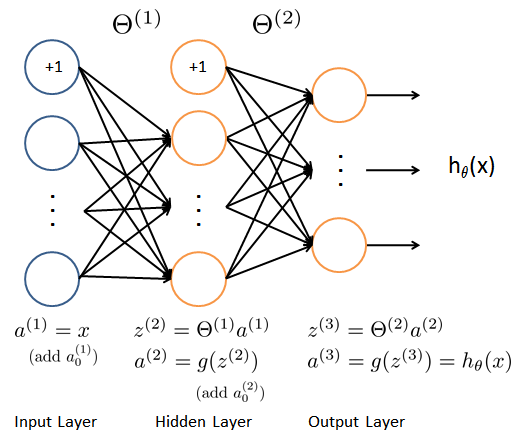
\includegraphics[width=0.65\textwidth]{img/redeneuralmulticlass}
\legend{Fonte: \citeonline{machinelearningcoursera}}
\end{figure}

O vetor de hipóteses resultante para um conjunto de entradas pode parecer como:
\begin{equation}
h_{\theta}(x) = \begin{bmatrix} 0 \\ 0 \\ 1 \\ 0 \end{bmatrix} \nonumber
\end{equation}

No qual a classe resultante é a terceira linha, ou $h_{\theta}(x)_3$. É possível extender essa definição para definir todo o conjunto de classes resultados como $y'$:
\begin{equation}
y^{(i)} = \begin{bmatrix} 1 \\ 0 \\ 0 \\ 0 \end{bmatrix} \begin{bmatrix} 0 \\ 1 \\ 0 \\ 0 \end{bmatrix} \begin{bmatrix} 0 \\ 0 \\ 1 \\ 0 \end{bmatrix} \begin{bmatrix} 0 \\ 0 \\ 0 \\ 1 \end{bmatrix} \nonumber
\end{equation}

E o valor final da hipótese para um conjunto de entrada será um dos elementos em $y$.


\subsection{Função de custo}

As subseções anteriores mostraram como representar uma rede neural, agora estamos interessados em como realizar a aprendizagem para resolver o problema de classificação.

Antes de apresentar a função de custo para redes neurais, será definido algumas variáveis úteis nesse escopo. Elas estão na \autoref{tab:tabfuncaocustorn}.

\begin{table}[!htb]
\begin{center}
\caption{Notação utilizada para aprendizado em redes neurais} \label{tab:tabfuncaocustorn}
\begin{tabular}{m{2cm}m{12.0cm}}
  \toprule
  $L$ 	& número total de camadas na rede\\
  $S_l$	& número de unidades (sem o viés de entrada) na camada $l$ \\
  $K$   & número de unidades de saída ou número de classes  \\
  \bottomrule
\end{tabular}
\end{center}
\end{table}

Na \autoref{subsec:clasmultirn} foi visto que é possível ter vários nodos de saída. É denotado $h_{\theta}(x)_k$ como sendo uma hipótese que resulta na k-ésima saída.

A função de custo para redes neurais é um pouco mais complicada que a utilizada na regressão logística, na verdade, ela é uma generalização da \autoref{eq:funcaodecustofinalreg}. 

Na \autoref{eq:funcaodecustorn}, foi adicionado alguns somatórios aninhados para tratar os múltiplos nodos de saída. Na primeira parte da equação, entre os colchetes, foi adicionado um somatório aninhado que itera sobre o número de nodos de saída.

Na parte da regularização (após os colchetes), foi lidado com as múltiplas matrizes $\theta$s. Conforme a regra \ref{eq:regradimensoes}, o número de colunas de uma dada matriz $\theta$ é igual ao número de nodos na camada atual (incluindo o viés). Já o número de linhas da matriz $\theta$ é igual ao número de nodos na próxima camada (sem o viés). 

\begin{equation}\label{eq:funcaodecustorn}
J(\theta) = \frac{-1}{m}\Big[ \sum\limits_{i=1}^m \sum\limits_{k=1}^K y_k^{(i)}log(h_{\theta}(x^{(i)})_k) + (1 - y_k^{(i)})log(1 - h_{\theta}(x^{(i)})_k) \Big] +
\frac{\lambda}{2m} 
\sum\limits_{l=1}^{L-1}
\sum\limits_{i=1}^{S_l}
\sum\limits_{j=1}^{S_{l+1}} (\theta_{j,i}^{l})^2
\end{equation}


\subsection{Algoritmo \textit{Backpropagation}}

Em redes neurais, para realizar a minimização de custo um dos algoritmos amplamente utilizado é o \textit{Backpropagation}. Seu objetivo é calcular as derivadas parciais da função de custo, para que depois seja possível realizar a operação: $min_{\theta}J(\theta)$. Ou seja, o objetivo é minimizar a função de custo $J$ usando um conjunto ótimo de parâmetros $\theta$. E para isso é necessário o cálculo da derivada parcial da função de custo em relação aos parâmetros $\theta$ para cada nodo de ativação em uma camada $l$, conforme mostrado na \autoref{eq:derivadabackprop}.

\begin{equation}\label{eq:derivadabackprop}
\frac{\partial}{\partial\theta_{i,j}^{(l)}} J(\theta)
\end{equation}


Em \textit{Backpropagation} é calculado o \textbf{erro} para cada nodo. Extendemos a notação usada pela \autoref{tab:tabfuncaocustorn} ao adicionar uma nova variável $\delta_j^{l}$ que é igual ao ``erro'' do nodo $j$ na camada $l$. Sendo assim, para a última camada, é possível calcular um vetor de valores $\delta$ com: $\delta^{(L)} = a^{(L)} - y$. Ou seja, os ``valores de erro'' para a última camada são simplesmente a diferença entre os resultados atuais na última camada e as saídas corretas em $y$.

A questão chave desse algoritmo é como obter os valores de $\delta$ nas camadas anteriores à última. Para isso é usado a \autoref{eq:deltaanteriores} que nos leva para trás, da direita para esquerda.

\begin{equation}\label{eq:deltaanteriores}
\delta^{(l)} = ((\theta^{(l)})^T \delta^{(l+1)}) .* g'(z^{(l)}))
\end{equation}

Os valores de $\delta$ da camada $l$ são calculados ao multiplicar os valores de $\delta$ na próxima camada com a matriz $\theta$ na camada $l$. Isso é multiplicado elementarmente com uma função $g'$, a qual é a derivada da função de ativação $g$ avaliada com os valores de entrada dados por $z^{(l)}$. A função $g'$ pode ser descrita como na \autoref{eq:funcaogprime}.

\begin{equation}\label{eq:funcaogprime}
g'(z^{(l)}) = a^{(l)} .* (1 - a^{(l)}) 
\end{equation}
\legend{Fonte: \citeonline{machinelearningcoursera}}

Portanto, a equação completa de \textit{Backpropagation} para os nodos interno é mostrada na \autoref{eq:backpropagationfinal}.

\begin{equation}\label{eq:backpropagationfinal}
\delta^{(l)} = ((\theta^{(l)})^T \delta^{(l+1)}) .* a^{(l)} .* (1 - a^{(l)}) 
\end{equation}

Agora é possível computar a derivada parcial ao multiplicar os valores de ativação e os valores de erro para cada exemplo de treinamento $t$, conforme mostrado na \autoref{eq:parcialbackpropfinal}.

\begin{equation}\label{eq:parcialbackpropfinal}
\frac{\partial}{\partial\theta_{i,j}^{(l)}} J(\theta) = \frac{1}{m} \sum\limits_{t=1}^{m} a_j^{(t)(l)} \delta_i^{(t)(l+1)}
\end{equation}

Isso porém ignora a regularização, que é feita depois.

Uma observação importante é que $\delta^{(l+1)}$ é um vetor com $S_{l+1}$ elementos, e $a^{(l)}$ é um vetor com $S_l$ elementos. Portanto a multiplicação deles vai gerar uma matriz com dimensão $S_{l+1} \times S_l$, que é a mesma dimensão que $\theta^{(l)}$. Ou seja, o processo irá produzir um termo gradiente para todos elementos em $\theta^{(l)}$. O algoritmo \ref{backpropalgorithmx} junta todas essas equações.

\begin{algorithm} 
\caption{Algoritmo de Backpropagation} \label{backpropalgorithmx}
\begin{algorithmic}
\Procedure{Backpropagation}{}
	\State dado um conjunto de treinamento $\{(x^{(1)}, y^{(1)}), \ldots, (x^{(m)}, y^{(m)}) \}$
	\State $\Delta_{i,j}^{(l)} = 0$ para todo $(l, i, j)$
	\For{cada exemplo de treinamento $t=1$ até $m$ }
		\State $a^{(1)} = x^{(t)}$
		\State \textit{Forward-Propagation}($a^{(2)}$)
		\State $\delta^{(L)} = a^{(L)} - y^{(t)}$
		\For{$l=L-1$ até $2$}
      \State $\delta^{(l)} = ((\theta^{(l)})^T \delta^{(l+1)}) .* a^{(l)} .* (1 - a^{(l)})$
		  \State $\Delta^{(l)} = \Delta^{(l)} + \delta^{(l+1)}(a^{(l)})^T $
    \EndFor
	\EndFor
		\If {$j = 0$}
			\State $D_{i,j}^{(l)} = \frac{1}{m}\Delta^{(l)}$
		\Else
			\State $D_{i,j}^{(l)} = \frac{1}{m}(\Delta^{(l)} + \lambda\theta^{(l)})$
		\EndIf
\EndProcedure
\end{algorithmic}
\end{algorithm}

A matriz $\Delta$ é usada apenas como um acumulador, com o intuito de passar adiante os valores enquanto é computado a derivada parcial. Os termos $D_{i,j}^{(l)}$ são as derivadas parciais finais, ou seja, os resultados esperados. A \autoref{fig:backpropagationalgex} ilustra os passos do algoritmo de \textit{Backpropagation} para uma rede neural com uma camada oculta.

\begin{figure}
\centering
\caption{Passos do Backpropagation} \label{fig:backpropagationalgex}
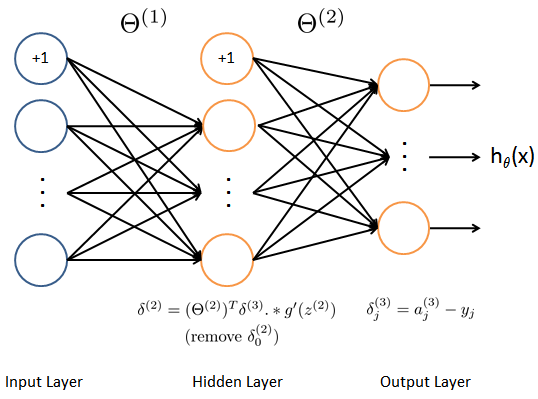
\includegraphics[width=0.65\textwidth]{img/backpropagationalg}
\legend{Fonte: \citeonline{machinelearningcoursera}}
\end{figure}

Segundo \cite{machinelearningcoursera}, uma observação importante a ser feita é que os pesos $\theta$ não podem ser inicializados com zero, pois isso não funciona em redes neurais. Uma solução para esse problema é realizar uma \textbf{inicialização aleatória} dos pesos.

\subsection{Treinamento}

Para treinar a rede, é necessário primeiramente escolher uma arquitetura (\textit{layout}) da rede neural, incluindo quantas unidades ocultas em cada camada e quantas camadas no total.

\begin{itemize}
	\item Número de unidades de entrada: igual ao número de dimensões das \textit{features} $x^{(i)}$;
	\item Número de unidades de saídas: igual ao número de classes $|y|$;
	\item Número de camadas ocultas: por padrão é 1, caso seja mais que isso, então deve ter a mesma quantidade de unidades de ativação em cada camada oculta.
\end{itemize}

Para treinar a rede neural, é possível seguir os seguintes passos:

\begin{enumerate}

\item Inicializar aleatóriamente os pesos $\theta$;
\item Implementar o \textit{Forward-propagation} para obter $h_\theta(x^{(i)})$;
\item Implementar a função de custo;
\item Implementar o \textit{Backpropagation} para computar as derivadas parciais;
\item Usar o Gradiente Descendente ou outro algoritmo de otimização para minimizar a função de custo com os pesos $\theta$.

\end{enumerate}


\section{Aprendizagem profunda}

A aprendizagem profunda é uma ramificação da aprendizagem de máquina, que baseia-se num conjunto de algoritmos que procuram modelar abstrações de alto nível usando modelos arquitetoriais, com estruturas complexas, compostas de múltiplas transformações não lineares \cite{deng2014deep}. Suas definições são intrínsecas, pois não há um consenso de quão profundo um modelo neural precisa ser para ser considerado um modelo de aprendizagem profunda. Entretanto, há a certeza de que aprendizagem profunda pode ser seguraramente categorizada como o estudo de modelos que tratam uma grande quantidade de composições de aprendizagem ou conceitos de aprendizagem que não conseguem ser empregados em aprendizado de máquina \cite{Bengio-et-al-2015-Book}. 

% A \autoref{fig:differentareas} demonstra a relação entre diferentes disciplinas de inteligência artificial (IA).

% \begin{figure}
% \centering
% \caption{Relações entre diferentes disciplinas em IA} \label{fig:differentareas}
% 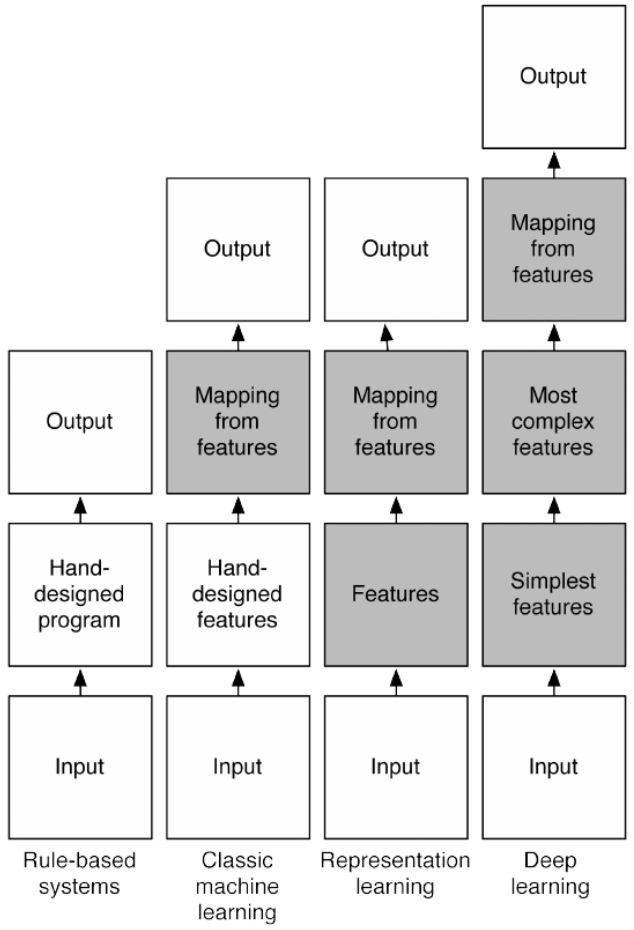
\includegraphics[width=0.65\textwidth]{img/differentareas}
% \legend{Fonte: \citeonline{Bengio-et-al-2015-Book}}
% \end{figure}


Extrair \textit{features} significantes manualmente é uma tarefa muito difícil, pois pode haver muitas variações nos dados que podem ser identificadas utilizando um nível sofisticado, quase humano, de entendimento. Quando é assim tão difícil de obter uma representação como de resolver o problema principal, a aprendizagem de representação parece não ajudar. 

Aprendizagem profunda resolve esse problema de representação ao introduzir representações que são expressas em termos de representações mais simples. Permitindo o computador a construir conceitos complexos a partir de conceitos simples. A \autoref{fig:aprendendodeep} ilustra um modelo de aprendizagem profunda.

\begin{figure}
\centering
\caption{Modelo de aprendizagem profunda} \label{fig:aprendendodeep}
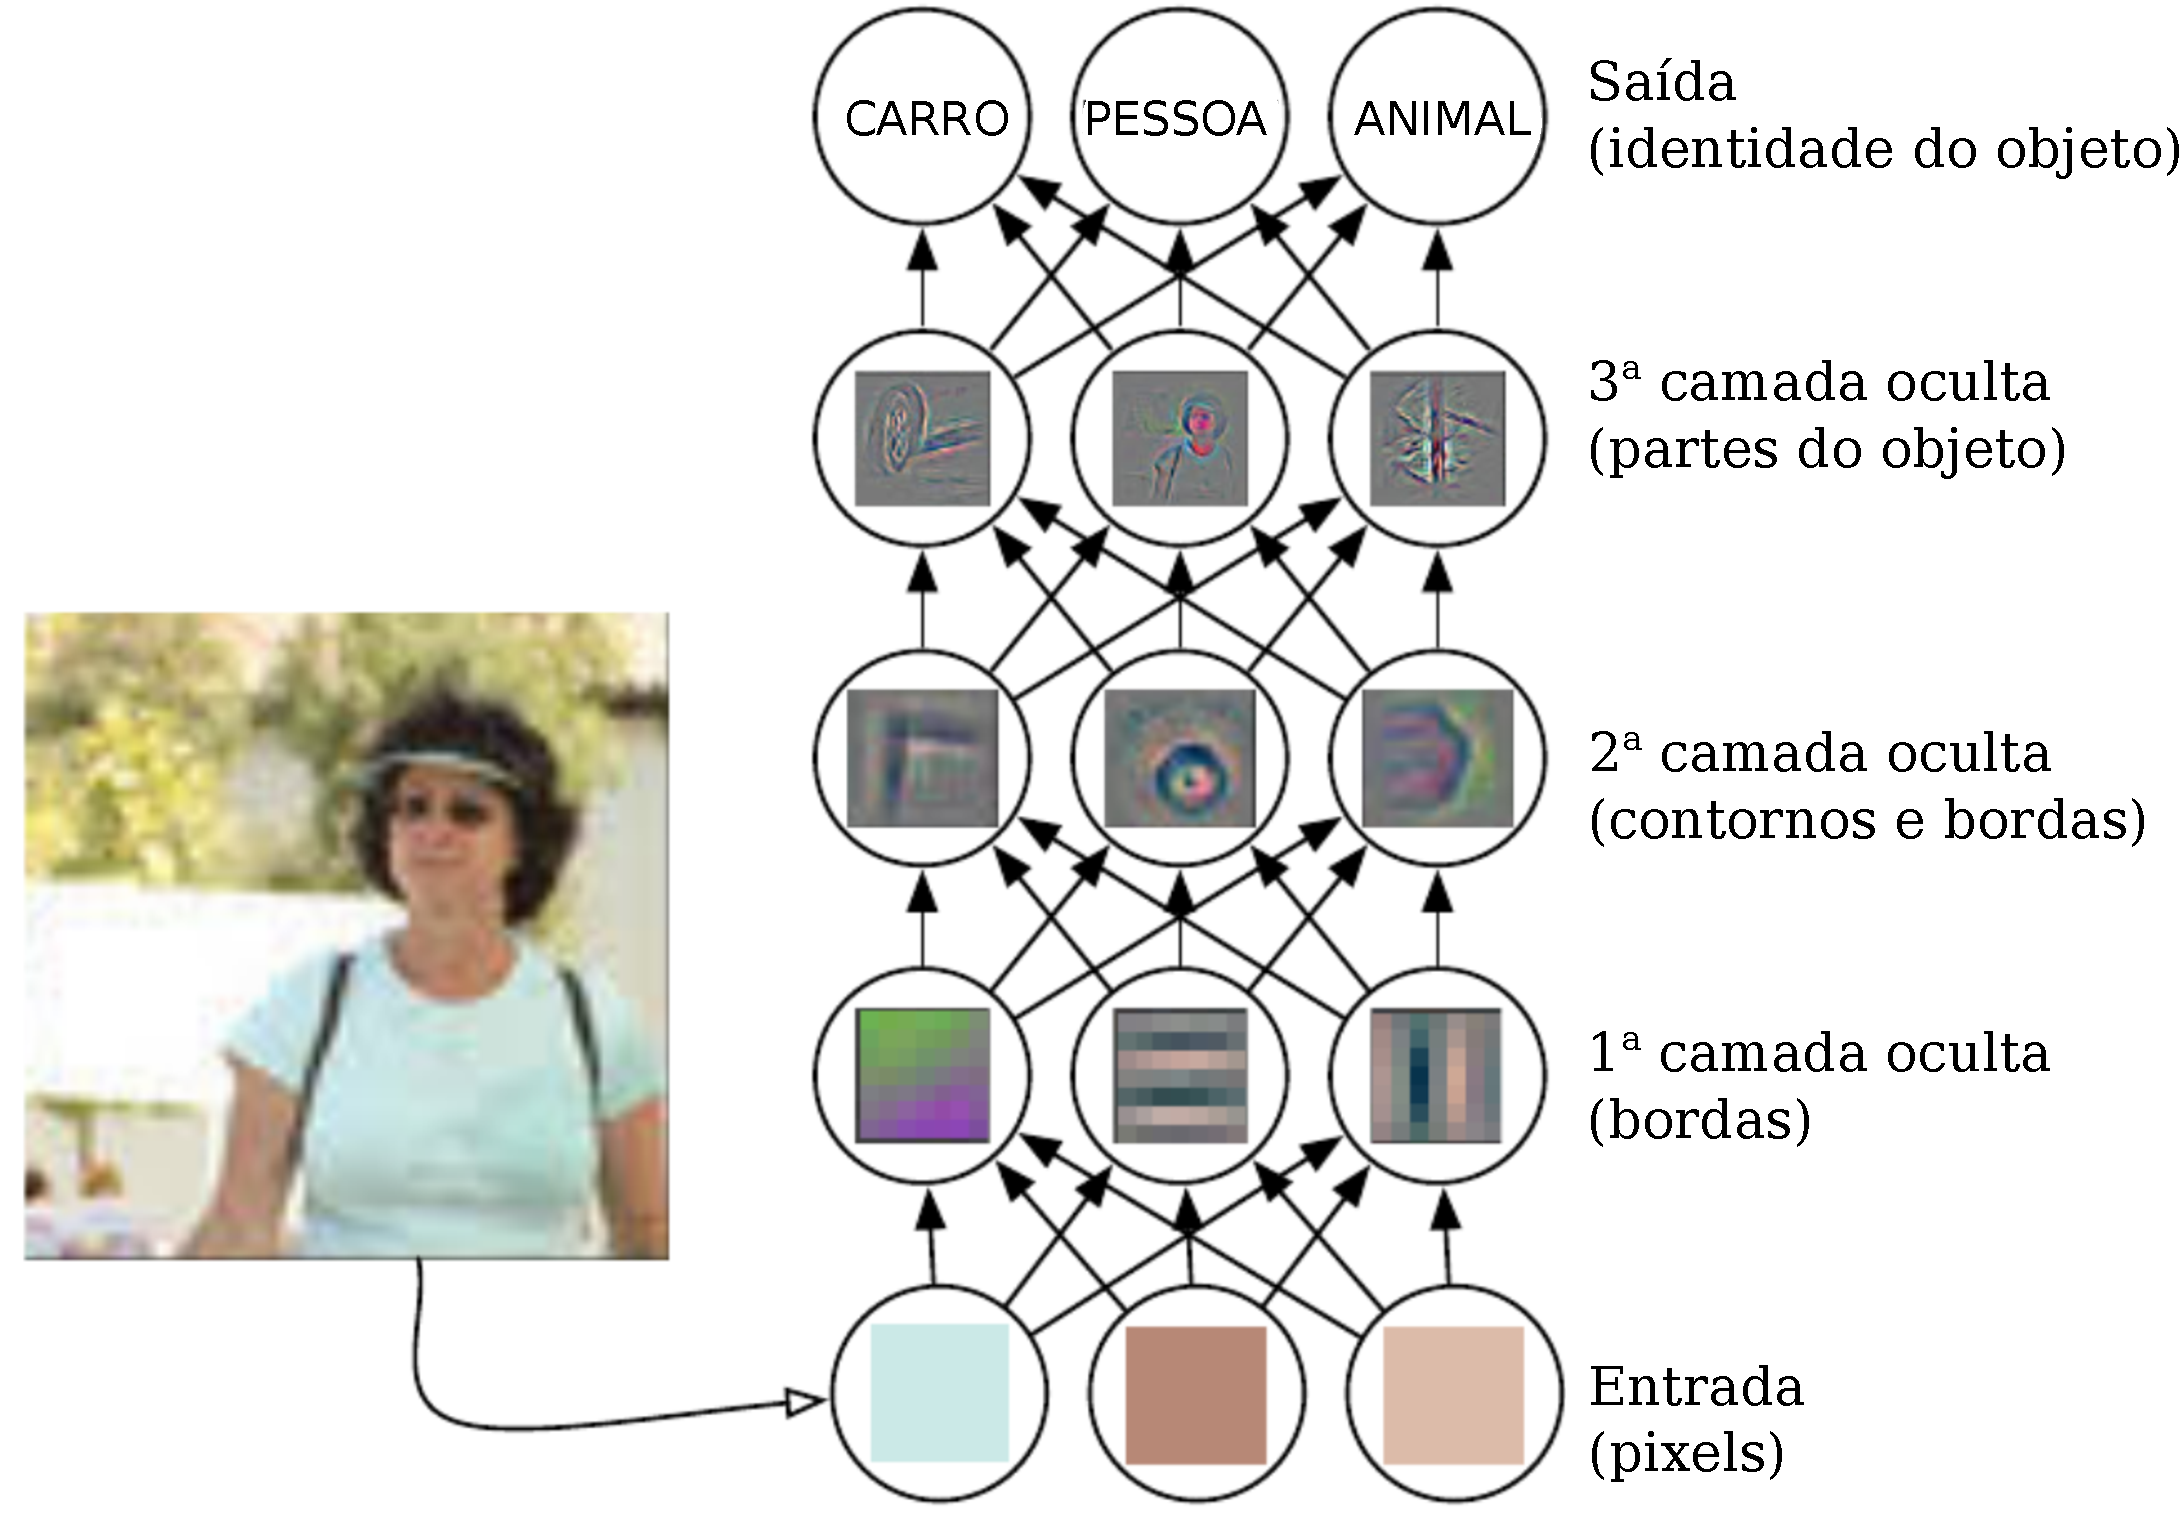
\includegraphics[width=0.75\textwidth]{img/aprendendodeep.pdf}
\legend{Adaptade de: \citeonline{Bengio-et-al-2015-Book}}
\end{figure}

Na \autoref{fig:aprendendodeep}, cada \textit{pixel} da imagem são \textit{features} passadas para a primeia camada oculta, que consegue identificar bordas facilmente ao comparar o brilho de \textit{pixels} vizinhos. Ao passar a descrição dessas bordas para a segunda camada oculta, ela consegue facilmente procurar por contornos, que são reconhecidos como uma coleção de bordas. Ao chegar na terceira camada oculta, consegue-se detectar partes inteiras de objetos específicos ao procurar por específicas coleções de contornos e bordas. No final, a descrição da imagem em termos das partes dos objetos pode ser usada para reconhcer objetos inteiros presentes na imagem \cite{Bengio-et-al-2015-Book}.


A \autoref{fig:sentidoadm} mostra que o aprendizado de máquina se resume em otimizar pesos para fazer uma ótima predição final. E para isso, é necessário dois itens: Descrever os dados através de \textit{features} de modo que o computador consiga entender; Aplicar um algoritmo de aprendizagem. Para o primeiro item, é necessário conhecimento do domínio específico, o que acaba gerando o chamado \textit{engenharia de features}, que ultimamente não é bem visto pela comunidade de \ac{pln}. O segundo item consiste em otimizar os pesos de acordo com as \textit{features}, e qualquer bom algoritmo de minimização da função de custo pode ser utilizado.

\begin{figure}
\centering
\caption{Sentido do aprendizado de máquina} \label{fig:sentidoadm}
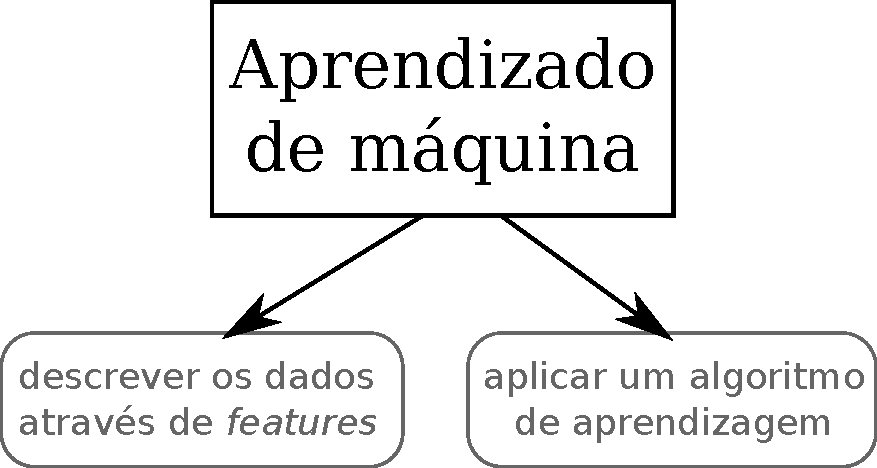
\includegraphics[width=0.75\textwidth]{img/sentidoadm}
\end{figure}

A aprendizagem profunda tenta automaticamente aprender boas \textit{features} ou representações. Na \autoref{sec:representacaodaspalavras} foi mostrado o conceito de \textit{word embeddings} ou vetor de \textit{features}, na verdade esse conceito está fortemente associado ao aprendizado profundo, onde tenta-se aprender múltiplos níveis da representação. Especificamente, é um tipo de aprendizado de máquina, uma técnica que permite sistemas computacionais à melhorarem com experiência e dados \cite{Bengio-et-al-2015-Book}.

O modelo dominante em aprendizado profundo é redes neurais. Nesse modelo, as \textit{features} são aprendidas rapidamente e automaticamente, adaptando-se muito bem as tarefas de \ac{pln}. Com isso, é possível aprender representações das informações linguísticas de modo não supervisionado (a partir do texto fonte) e também de modo supervisionado (usando classes específicas). Ela começou a ser usada recentemente devido a criação de novos modelos, algoritmos e ideias, e também devido ao aumento do desempenho computacional \cite{deeplearningfornlp}.

\begin{figure}
\centering
\caption{Tamanho das redes neurais ao longo dos anos} \label{fig:aumentorntam}
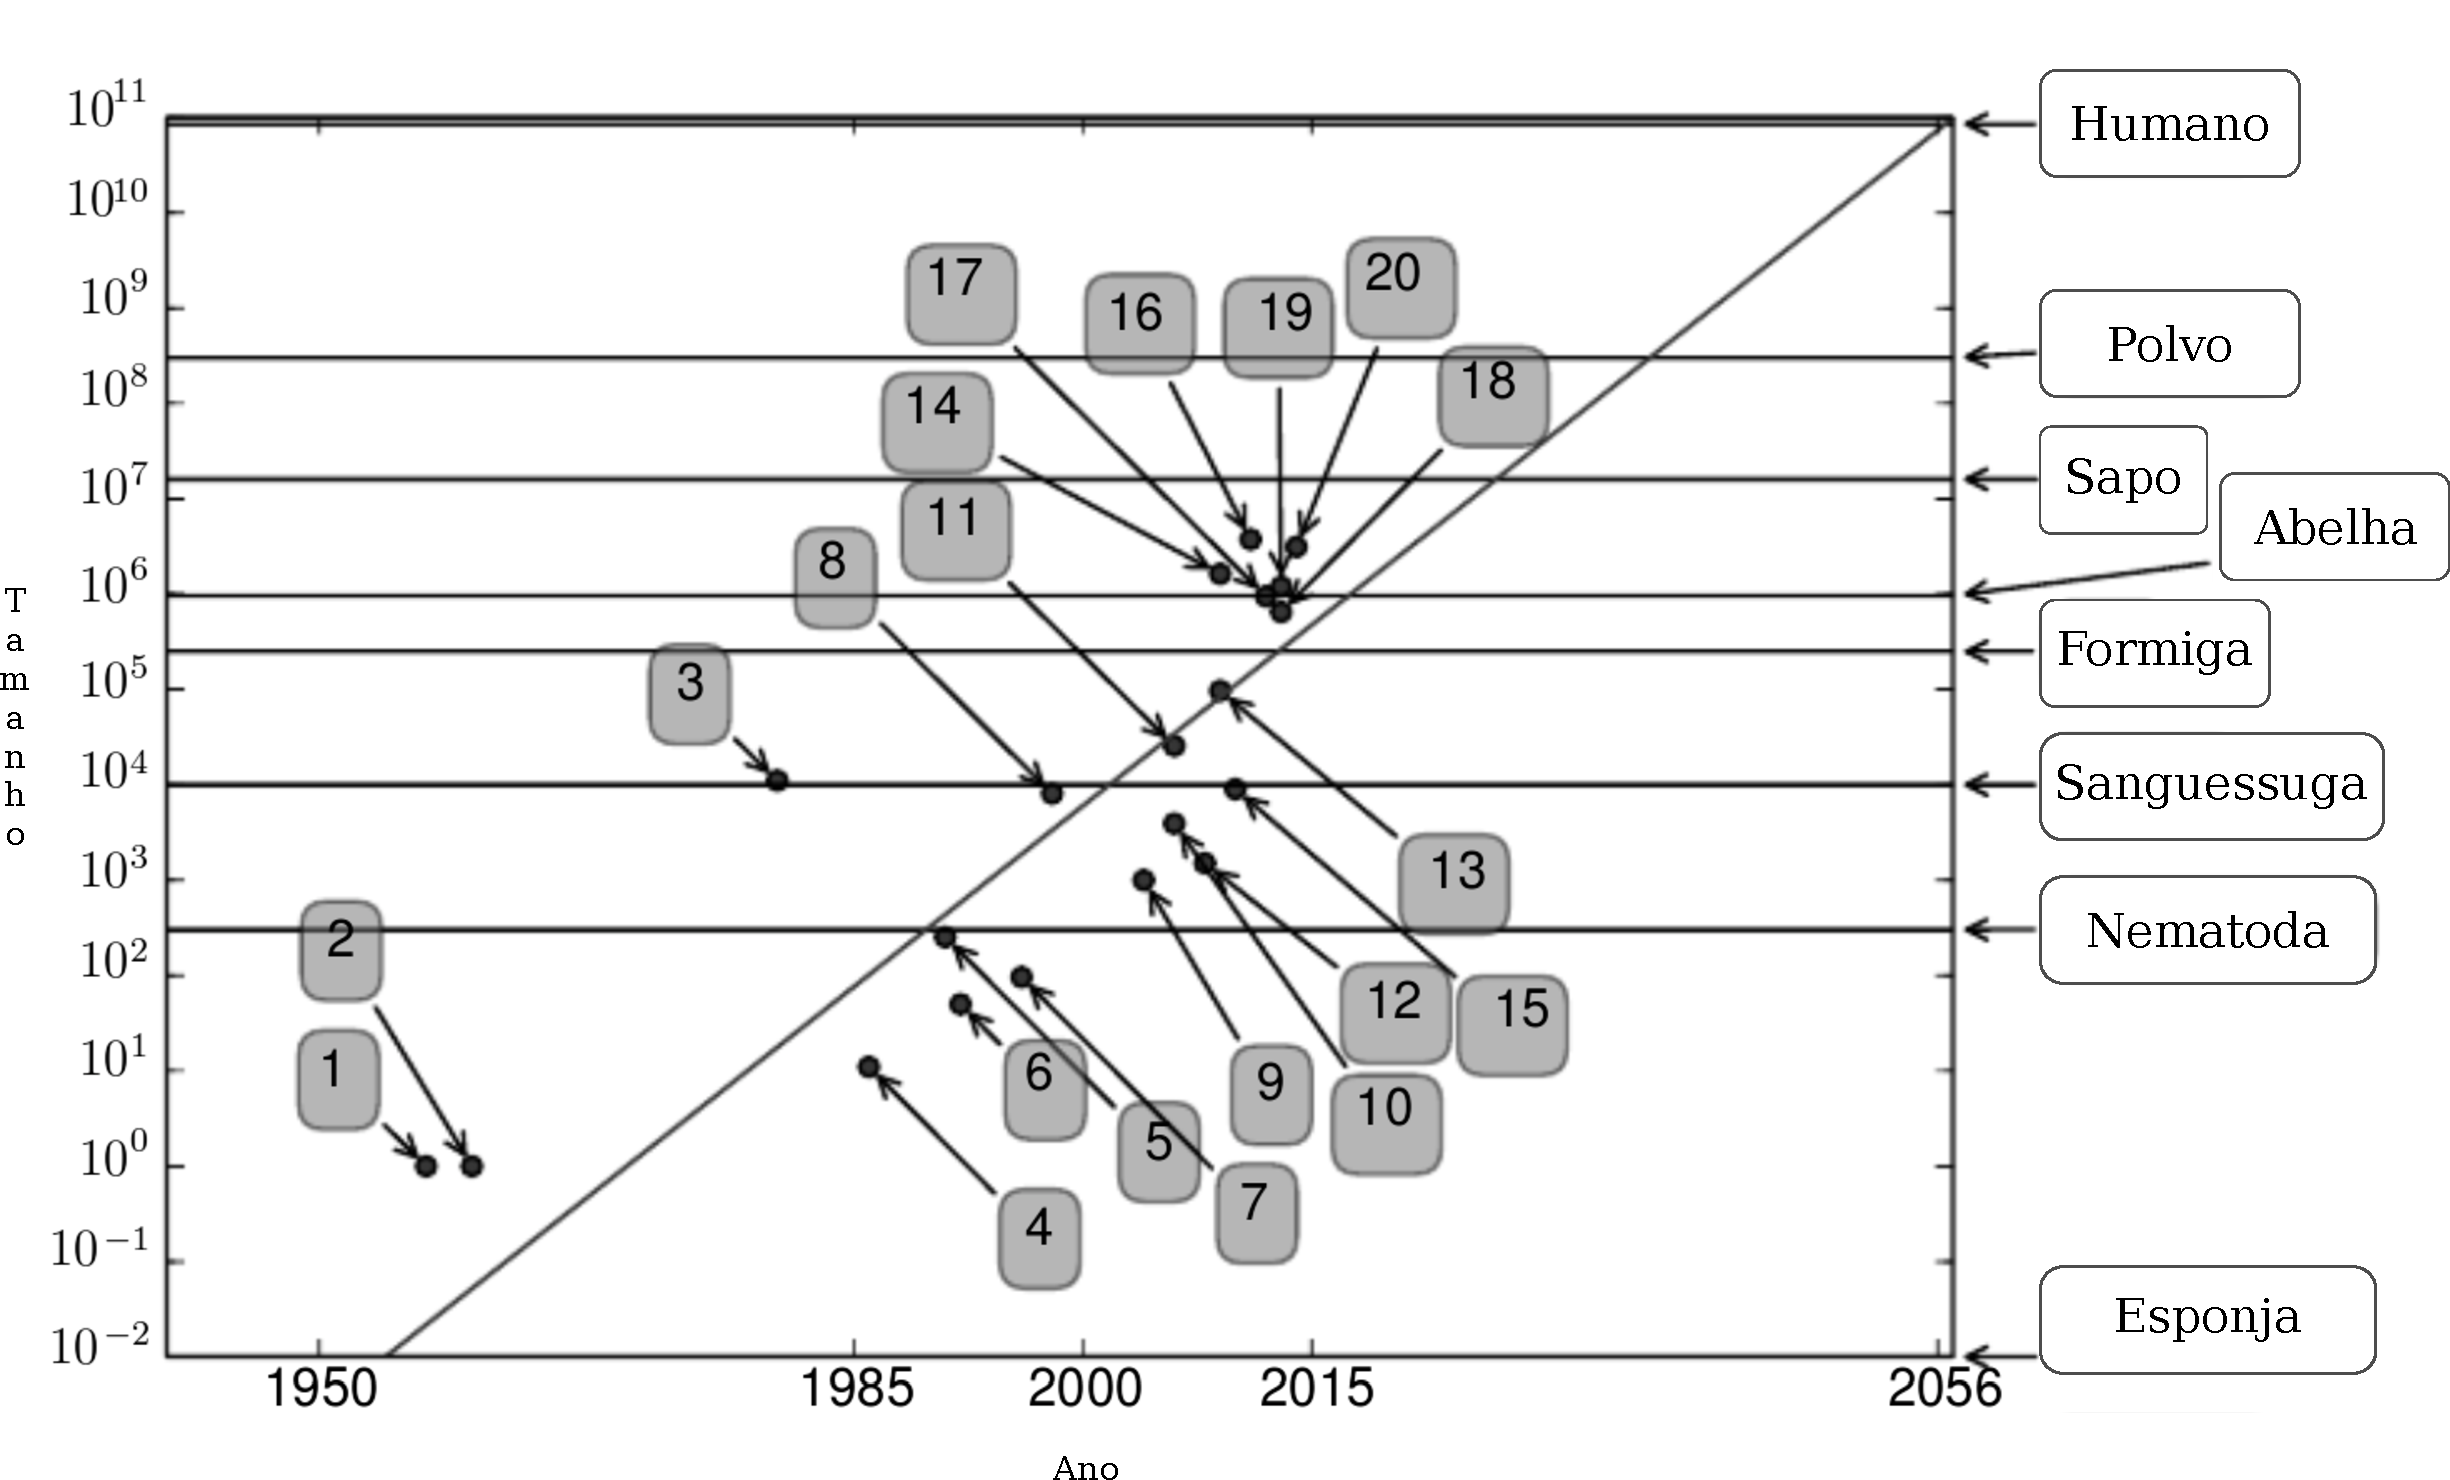
\includegraphics[width=0.75\textwidth]{img/aumentorntam.pdf}
\legend{Adaptade de: \citeonline{Bengio-et-al-2015-Book}}
\end{figure}

Como o processo de criação automatizada de \textit{features} acaba gerando muitos vetores de representações, temos que criar um modelo capaz de trabalhar com essas informações com o objetivo de aprender. Por isso, geralmente se trabalha com redes neurais com múltiplas camadas. A \autoref{fig:aumentorntam} demonstra o aumento do tamanhos das redes neurais de acordo com o tempo. 

A técnica utilizada ultimamente em \ac{pos} Tagging está ilustrada na \autoref{fig:atualmentepost}. Que consiste em primeiramente obter a representação das palavras em vetores reais com dimensões definidas pelo usuário, e após isso mesclar com \textit{features} de formato das palavras (e.g capitalização), para então jogar esses vetores como entrada numa rede neural. O que muda em cada abordagem geralmente é a questão do treinamento da representação das palavras, as novas \textit{features} criadas e como é organizado o modelo da rede neural.

\begin{figure}
\centering
\caption{Funcionamento de aprendizagem profunda em \ac{pos} Tagging} \label{fig:atualmentepost}
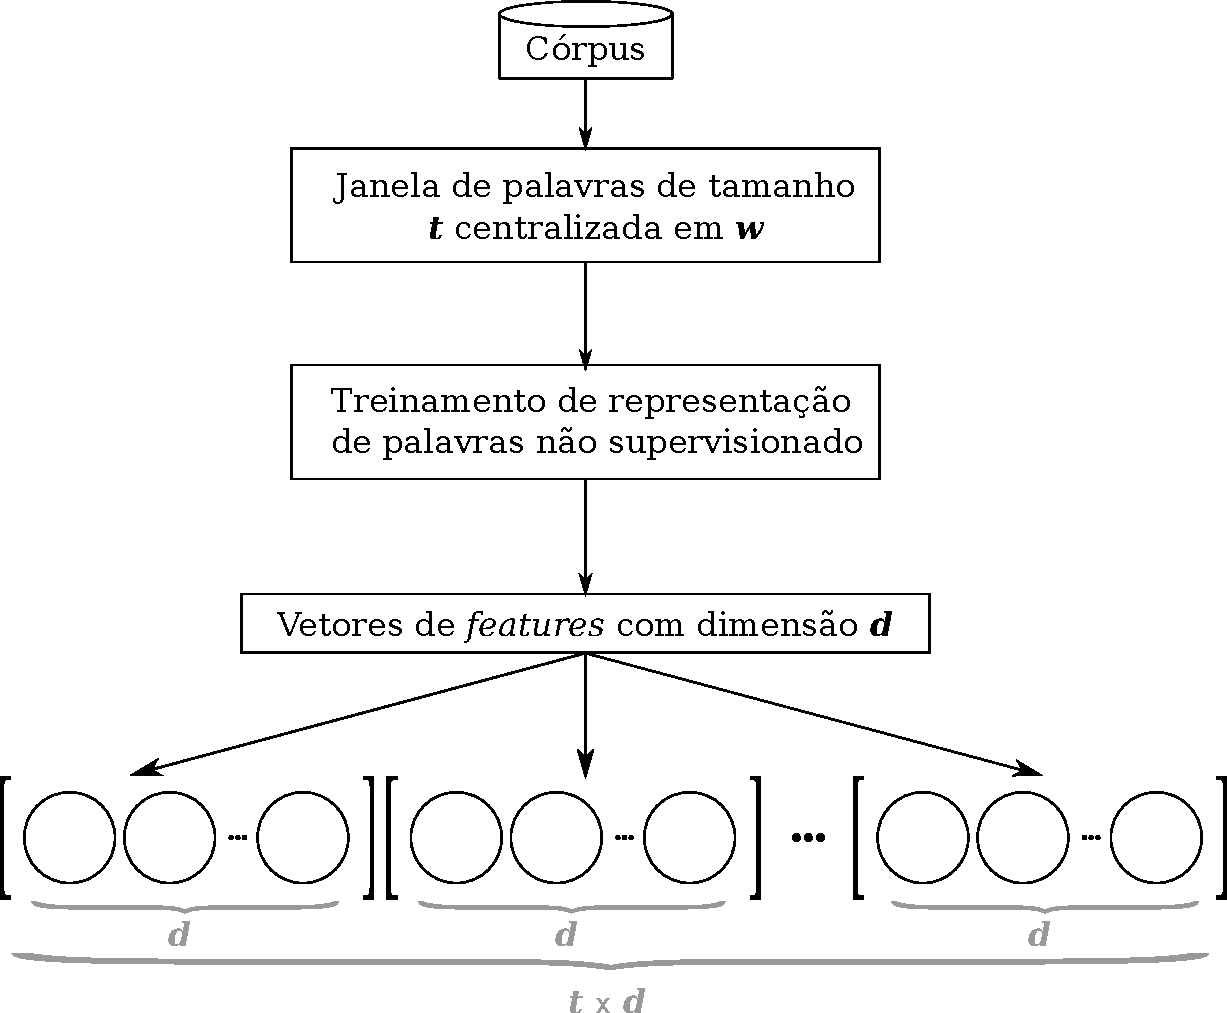
\includegraphics[width=0.75\textwidth]{img/deeplearningfunc}
\end{figure}

